%%==================================================
%% chapter03.tex for SJTU Master Thesis
%% based on CASthesis
%% modified by wei.jianwen@gmail.com
%% version: 0.3a
%% Encoding: UTF-8
%% last update: Dec 5th, 2010
%%==================================================

% \bibliographystyle{sjtu2} %[此处用于每章都生产参考文献]

\chapter{链路质量测试与建模}
\label{chap:delivery}

本章针对移动802.11n网络中链路质量测试与建模,首先给出目前移动802.11n网络链路质量测试存在的主要问题,包括移动网络的链路质量测试以及MIMO-OFDM系统多配置所带来的PDR-RSS模型过渡窗口问题;然后针对移动网络链路质量的时空变化特性,提出动态滑动平均算法,以提高链路质量测试精度并降低测试开销;同时针对MIMO-OFDM系统PDR-RSS模型的过渡窗口问题,提出在线PDR-RSS建模框架,以提高MIMO-OFDM配置选择效率;最后给出算法设计及系统实现,并对以上算法进行性能评估。

\section{问题描述}
\label{sec:problem3}

无线网络的一个基本问题是系统的可靠性与传输性能的合理平衡,其中信道状态和链路质量既是衡量网络性能的重要指标,又是系统决策的关键状态变量,因此信道状态和链路质量的测试与建模无线系统性能具有重要影响。

\subsection{现有工作}
\label{sec:current3}

\begin{figure}[!htp]
\centering
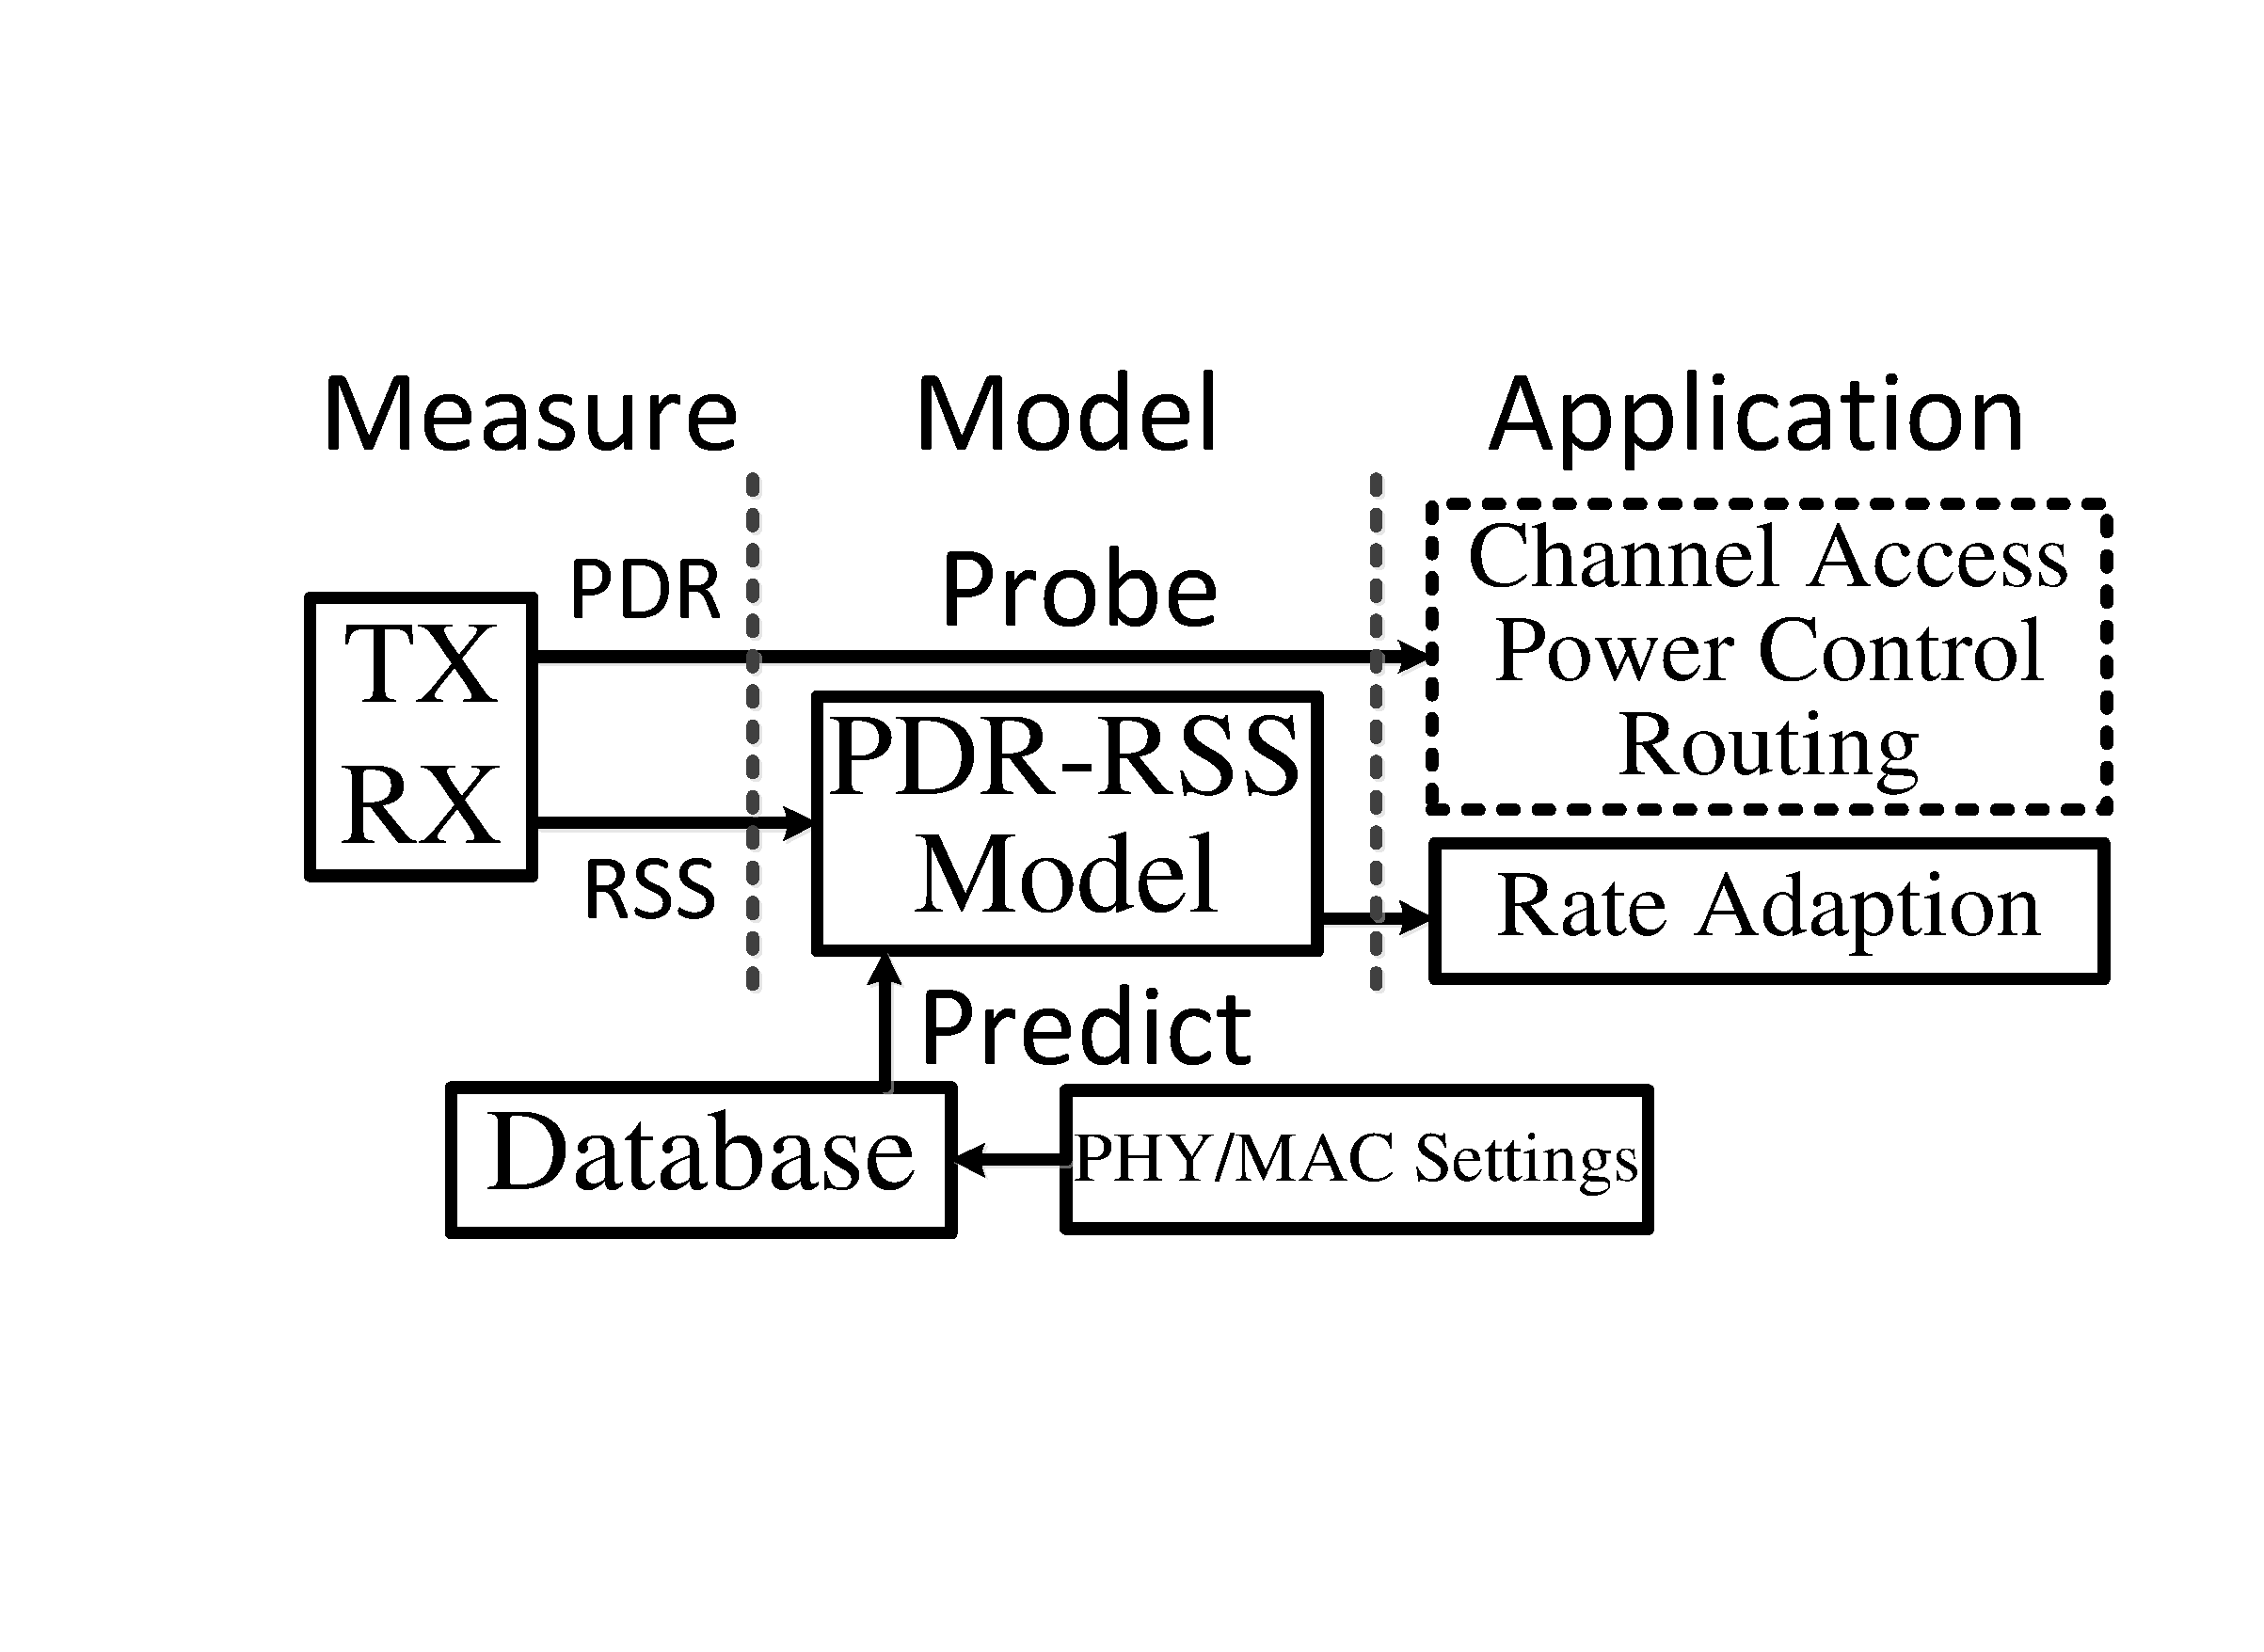
\includegraphics[width=0.6\textwidth]{chap3/modeling1.pdf}
\bicaption[fig:offlinemodel]{静态链路质量-信道状态模型}{静态链路质量-信道状态模型}{Fig}{General static PDR-RSS modeling framework}
\end{figure}

传统无线网络的上层应用,包括速率适配、功率控制及路由策略等,都不可避免地需要底层的网络状态信息,比如物理层信道状态或链路层链路质量。图 \ref{fig:offlinemodel} 所示为基于静态PDR-RSS模型的应用框架,本文中以速率控制为例进行详细介绍。从图中可以看出,基于静态PDR-RSS模型的速率控制算法主要分为两类:第一类通过探测数据包对链路层链路质量进行实时测试,直接根据当前链路质量进行速率选择;第二类利用静态PDR-RSS模型,根据当前物理层信道信息对网络状态进行预测,并作出相应配置选择。

以上的静态PDR-RSS框架无法之际应用于移动MIMO-OFDM系统中:第一,由于移动无线网络在运行过程中外界环境与网络状态复杂多变,从而降低链路质量的测试精度;第二,由于802.11n系统采用了多种物理层和链路层配置,从而增加了链路质量的测试开销;第三,MIMO-OFDM的多配置特性增加了PDR-RSS模型的复杂性\footnote{多种配置需要分别进行建模,同时MIMO-OFDM系统的PDR-RSS模型具有过渡窗口效应}。所以移动802.11n网络的移动性和多配置性降低了链路质量的测试与预测精度,进一步影响网络的整体性能。

\subsection{存在问题}
\label{sec:prob3}

本节通过大量实验数据说明以上静态框架应用于移动802.11n网络中存在的问题,从而引入移动MIMO-OFDM系统中链路质量测试与建模过程中存在的关键问题。静态PDR-RSS框架的主要特点包括:
\begin{itemize}
  \item 固定参数设定的PDR测试算法
  \item 静态PDR-RSS模型与数据库
  \item 单一测量与判决指标(PDR或RSS)输入
\end{itemize}
静态PDR-RSS框架的以上特点无法满足移动性带来的网络状态的时空变化,以及多配置带来的PDR-RSS模型的过渡窗口问题。

\begin{figure}[!htp]
\centering
    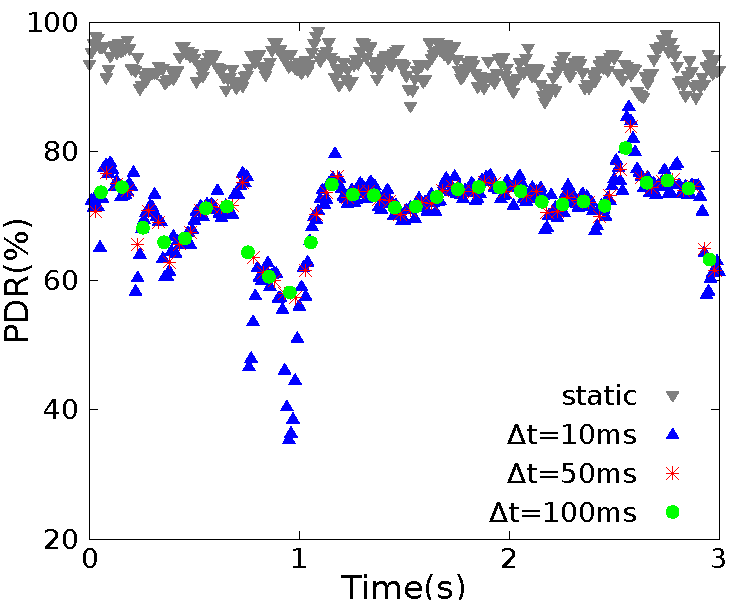
\includegraphics[width=0.8\textwidth]{chap3/pdrvary.pdf}
\bicaption[fig:pdrover]{链路质量测试误差}{链路质量测试误差}{Fig}{PDR overestimation as sudden decline}
\end{figure}

\begin{itemize}
  \item \textbf{移动网络时空特性:}
  移动网络的时空变化特性对PDR的测量精度与开销具有重要影响。无线网络中广泛应用指数加权平均算法进行链路质量测试 \upcite{ath9k} \upcite{minstrel} \upcite{wong2008wireless},一般其参数设置为固定值,比如采样周期一般设置为50ms或100ms,而加权因子一般设置为0.25或0.125。但是网络状态的时空变化会降低EWMA算法的测试精度,尤其当网络运行与较高数据传输速率时。图 \ref{fig:pdrover} 所示的实验结果说明了网络状态变化对PDR测试的影响,当被测PDR发生瞬时变化时,采样周期固定为50ms或100ms的EWMA算法无法获得准确的PDR信息,甚至出现20\%的测试误差。因此有必要对PDR测试算法进行改进,以提高移动网络中链路质量测试精度。现有的针对移动网络链路质量测试方法的工作主要针对RSS的测试 \upcite{chen2011ram} \upcite{judd2008efficient}。
  \item \textbf{MIMO-OFDM系统过渡窗口:}
  MIMO-OFDM系统的多种配置增加了链路质量测试与预测的复杂度。由于802.11n网络采用了多种物理层和链路层技术,同时网络运行时需要在多种配置见进行切换,从而增加了链路质量测试的复杂度,MIMO-OFDM系统中PDR-RSS模型的过渡窗口进一步增加了802.11n网络中PDR-RSS建模的复杂度 \upcite{Halperin2010predictable}。如图 \ref{fig:transition} 所示,802.11n网络的PDR-RSS模型存在3-15dB的过渡窗口长度,对于静态建模框架约有34\%的被选配置落入过渡窗口,甚至有8\%的配置位于过渡窗口左侧\footnote{落入过渡窗口表示PDR<$P_{thrh}$=90\%,位于过渡窗口左侧表示PDR<$P_{thrl}$=10\%}。因此有必要针对MIMI-OFDM系统的多配置特性,设计有效的PDR-RSS建模方法与配置选择策略。
\end{itemize}

\begin{figure}[!htp]
\centering
    \subfigure[PDR-RSS模型]{
    \label{fig:pdr-rss}
    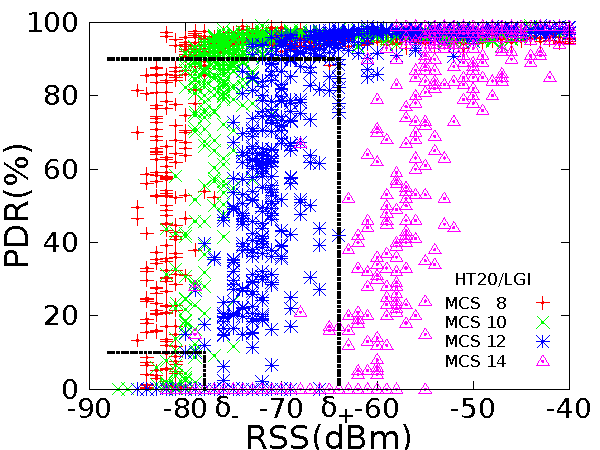
\includegraphics[width=0.46\textwidth]{chap3/pdr.pdf}}
    \hspace{1cm}
    \subfigure[过渡窗口]{
    \label{fig:MCS}
    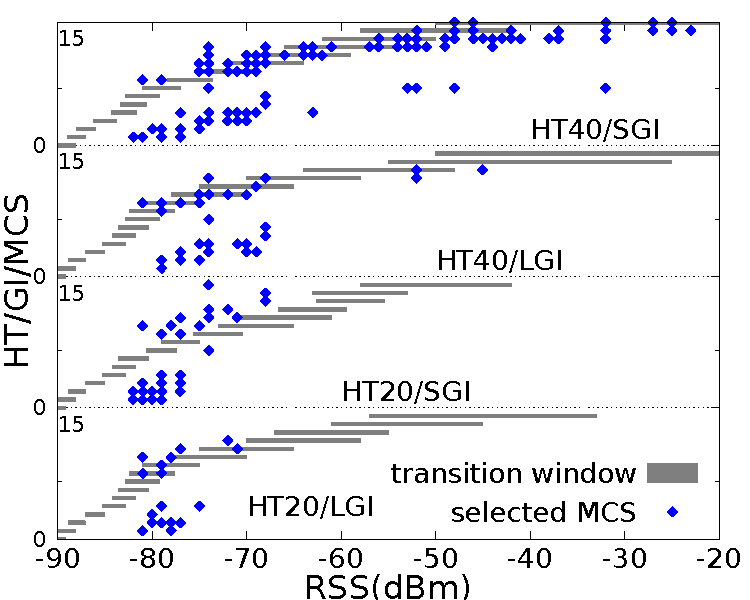
\includegraphics[width=0.44\textwidth]{chap3/MCS.pdf}}
\bicaption[fig:transition]{PDR-RSS模型过渡窗口}{PDR-RSS模型过渡窗口}{Fig}{Transition windows of PDR-RSS model as high data rates}
\end{figure}

802.11n网络的物理层和链路层配置一方面显著提升网络性能,但是同时使得链路质量测试与建模更为复杂。移动终端造成网络状态的时空变化特性,从而对链路质量测试的精度与开销提出更高要求。本文提出在线建模框架以有效解决一下问题:(1)动态链路质量测试算法;(2)在线PDR-RSS建模与实时更新机制;(3)高效准确的多配置选择策略。

\section{链路质量动态测试}
\label{sec:measure}

\subsection{信号传输模型}
\label{sec:packetmodel}

为了对不同的链路质量测试方法进行刻画,并对不同测试方法进行分析,首先引入数据包传输模型。发送数据包的接收状态可以认为是离散随机过程$X=\{x_1, x_2, ... x_i\}$,而每一个数据包的接收状态为0或1,即$x_i=\{0, 1\}$, $i(i=1,2,3...)$,其中$x_i=1$表示第$i$个数据包成功接收。第$i$个数据包成功接收的概率$\textbf{P(}x_i=1\textbf{)}=p_i$可以由标准的信噪比模型来刻画,如下式所示:
\begin{equation}
 p_i=\textbf{P(}SINR_i(t)>\delta\textbf{)}=\textbf{P(}\frac{R_i(t)}{I_i(t)+n}>\delta\textbf{)}
\label{equa:p_i}
\end{equation}
其中$SINR_i(t)$为第$i$个接收数据包在$t$时刻的信噪比,$\delta$为信噪比门限值,$R_i(t)$为接收数据包在时刻$t$的接收信号强度,$I_i(t)$ 为除传输信号外其他信号$R_j(t)$造成的接收端信号干扰,$n$为热噪声且一般为恒定值。同时$p_i$可以由实测模型表示,即
\begin{equation}
 p_i=\hat{p}(R_i(t))
\label{equa:p_i_measure}
\end{equation}
其中$\hat{p}(R_i(t))$为基于实测数据的传输成功率,表示为接收信号强度的函数。

\subsection{传统测试方法}
\label{sec:traditional}

\begin{figure}[!htp]
\centering
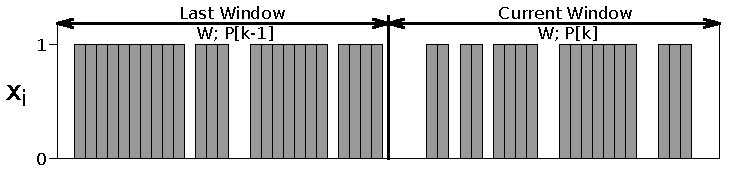
\includegraphics[width=5in]{chap3/m_weighted.pdf}
\bicaption[fig:weighted]{静态加权平均}{静态加权平均}{Fig}{EWMA with fixed $W$ and $\alpha$}
\end{figure}

对于静态无线网络中的传输成功率测试,在统计区间内的数据包的接收状态可以认为常数,且$x_i$为独立同分布的随机变量,即$P(x_i=1)=p_i=p$,此时$X$可以刻画为伯努利过程,即$X\sim B(p)$。一般采用固定窗口长度进行平均,如图 \ref{fig:weighted} 所示,第$k$次测试的传输成功率为
\begin{equation}
PDR_f[k]=\frac{1}{W}\sum_{i=kW+1}^{(k+1)W}{x_i}
\label{equa:pdr_f}
\end{equation}
其中$W$为平均窗口长度。此时的测试误差可以表示为测试传输成功率与接收成功概率的差,因此测试误差的期望与方差分别为:
\begin{equation}
 \textbf{E[}\Delta PDR_f\textbf{]}=\textbf{E[}\frac{1}{W}\sum_{i=1}^{W}{x_i}-p\textbf{]}=\frac{1}{W}\sum_{i=1}^{W}{\textbf{E[}x_i\textbf{]}}-p=0
\label{equa:Epf}
\end{equation}
\begin{equation}
 \textbf{D[}\Delta PDR_f\textbf{]}=\textbf{D[}\frac{1}{W}\sum_{i=1}^{W}{x_i}-p\textbf{]}=\frac{1}{W}\sum_{i=1}^{W}{\textbf{D[}x_i\textbf{]}}=p(1-p)
\label{equal:Dpf}
\end{equation}
其中$\overline{p}[k]$与$\overline{p'}[k]$分别为$P[k]$与$P'[k]$的估计值,可以由式(\ref{equa:Epf})获得,即
\begin{equation}
 \textbf{E[}P[\cdot]\textbf{]}=\frac{1}{N}\sum\textbf{E[}x_i\textbf{]}=\frac{1}{N}\sum{p_i}=\overline{p}[\cdot]
\label{equal:pestimation}
\end{equation}
其中$N$为窗口长度,$\overline{p}[\cdot]$为该统计区间内$p_i$的算术平均值,$p_n$当前时刻发送数据包的接收概率并作为传输成功率的真实值。从式(\ref{equal:pestimation})可以看出测试误差与$p_i$的变化情况密切相关,而$p_i$在静态无线网络与移动无线网络中呈现不同的特性。同时平均窗口长度$W$ 对于测试误差具有很大影响,例如当$p_i$在短时间尺度内出现剧烈变化时,过大的窗口长度会丢失传输成功率的细节信息。

在实际系统中一般采用指数加权平均,即EWMA算法,例如在Atheros's Linux系统的无线驱动中,包括针对802.11a/b/g网络的\texttt{Madwifi} \upcite{madwifi} 以及用于802.11n网络的\texttt{ath9k} \upcite{ath9k},以提高测试精度并降低测试开销。在EWMA中测试传输成功率表示为当前测试结果与历史结果的加权平均,即
\begin{equation}
 PDR_w[k]=\alpha PDR_f[k-1]+(1-\alpha)PDR_f[k]
\label{equal:pdr_w}
\end{equation}
其中$\alpha$为加权因子。此时EWMA的测试误差为:
\begin{equation}
\begin{split}
 \textbf{E[}\Delta PDR_w\textbf{]}&=\textbf{E[}\alpha PDR_f+(1-\alpha)PDR_f-p\textbf{]}\\
         &=\alpha \textbf{E[}PDR_f\textbf{]}+(1-\alpha)\textbf{E[}PDR_f\textbf{]}-p\\
         &=\alpha p + (1-\alpha) p-p\\
         &=0
\end{split}
\label{equa:Epw}
\end{equation}

\begin{equation}
\begin{split}
 \textbf{D[}\Delta PDR_w\textbf{]}&=\textbf{D[}\alpha PDR_f+(1-\alpha)PDR_f-p\textbf{]}\\
         &=\alpha^2\textbf{D[}PDR_f\textbf{]}+(1-\alpha)^2\textbf{D[}PDR_f\textbf{]}\\
         &=[\alpha^2+(1-\alpha)^2]p(1-p)
\end{split}
\label{equa:Dpw}
\end{equation}

从以上的分析可以看出,在静态无线网络传输成功率测试中,固定窗口与加权算法都可以获得无偏估计,而加权算法在不增加测试开销的前提下具有更低的均方差,由式(\ref{equa:Dpw})可以得出当$\alpha=0.5$时,理论上可以得到最小均方差$\textbf{D[}PDR_w\textbf{]}$。对于如图 \ref{fig:mobile_k} 中给定的接收成功概率$p\sim N(0.8, 0.01)$,相对于固定窗口测试方法,加权算法可以获得更准确的测试结果。如图 \ref{fig:static_e} 所示,固定窗口算法测试结果为80.23\%,而$\alpha=0.5$时的加权算法测试结果为80.06\%,可以看到两者的测试误差都很小,且固定窗口算法的均方差为0.0268,而加权算法在$\alpha=0.5$ 时的均方差为0.0034。

\begin{figure}[!htp]
\centering
\subfigure[原始平均 ($\alpha=0$)]{
    \label{fig:fixed_s}
    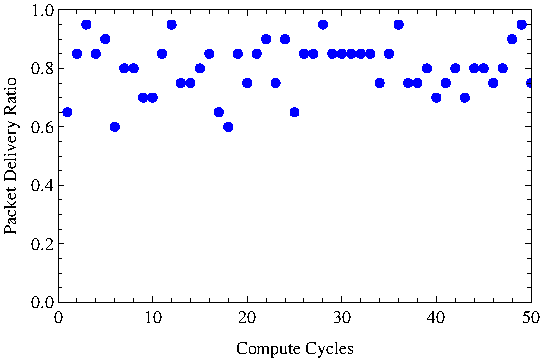
\includegraphics[width=2.5in]{chap3/fixed_n.pdf}}
    \hspace{1cm}
\subfigure[加权平均 ($\alpha=0.5$)]{
    \label{fig:weighted_s}
    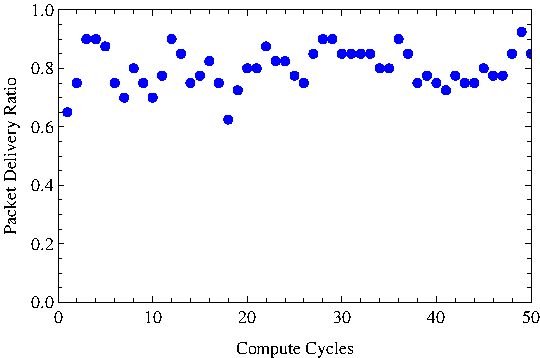
\includegraphics[width=2.5in]{chap3/weighted_n.pdf}}
\bicaption[fig:static]{静态网络测试精度}{静态网络测试精度}{Fig}{Measurement Window Length in Static Wireless Networks ($W=20, p=0.8$)}
\end{figure}

\begin{figure}[!htp]
\centering
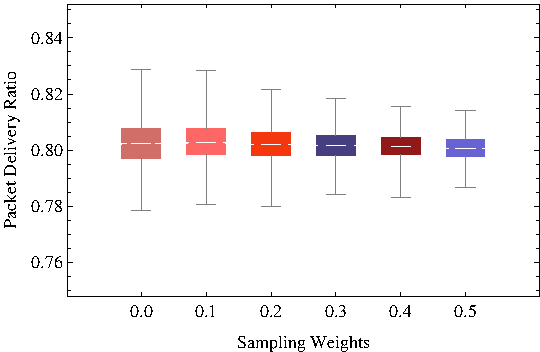
\includegraphics[width=5in]{chap3/static.pdf}
\bicaption[fig:static_e]{测试精度 ($\alpha=0\sim0.5$)}{测试精度 ($\alpha=0\sim0.5$)}{Fig}{Measurement Accuracy for Weighted Averaging}
\end{figure}

但是在实际测试中,加权因子$\alpha$一般在0.1到0.4之间取值,主要原因是$p_i$并不保持不变,而在移动无线网络中这种情况更为明显,因此当固定加权算法应用在移动无线网络测试中时,无法保证传输成功率的测试精度,从而影响网络性能,主要有以下原因:

\begin{itemize}
  \item 平均窗口长度以时间计量并为固定值,一般设置为50ms或100ms,难以对802.11n网络的多种配置进行有效测试;
  \item 合适的加权因子难以选择,理论上$\alpha$应设置在0.1到0.3之间 \upcite{EWMAChart},在实际中一般选择固定值0.125 \upcite{ath9k}或0.25 \upcite{minstrel}。
\end{itemize}

以上两点造成加权算法无法对测试精度与测试开销进行有效地控制,因此有必要针对移动802.11n网络的时空多变及多配置特性,提出有效地传输成功率测试算法,以适应链路质量的变化并有效调整测试精度与开销。

\subsection{动态滑动平均}
\label{sec:sliding}

对于移动无线网络传输成功率的测试而言,需要考虑测试精度与开销的权衡与折中问题。一方面其测量周期需要尽量短,以适应移动终端接收信号强度的突变并提高测试精度;另一方面在网络状态稳定或传输速率较低时,需要降低采样频率以减小对网络可用资源的影响并降低测试开销。

由于无线网络无线传播环境的复杂性,尤其对于移动网络与移动终端而言,造成接收信号强度和干扰的在传输成功率测量过程中的时空变化特性,使得数据包接收成功概率$p_i$在短时间尺度内变化;同时由于802.11n网络采用了MIMO-OFDM技术,造成其物理层与链路层的多配置特性,从而造成链路质量测试复杂性的升高及有效性的降低。因此有必要对原有加权算法进行改进,以适应移动网络的时空特性,并适应MIMO-OFDM系统的多配置特性。

\begin{figure}[!htp]
\centering
    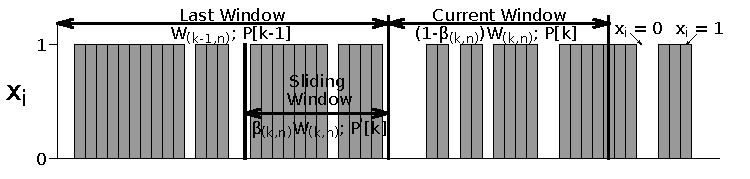
\includegraphics[width=5in]{chap3/m_sliding.pdf}
\bicaption[fig:sliding]{动态滑动平均}{动态滑动平均}{Fig}{DSWA with dynamic $W$ and $\beta$}
\end{figure}

针对以上问题,本文提出基于动态滑动窗口平均的传输成功率测试算法,如图 \ref{fig:sliding} 所示,当前测试窗口与上一测试窗口间存在重叠区域,即滑动窗口。在DSWA中PDR的测量值为
\begin{equation}
 \hat{P_s}[k]=\beta P'[k]+(1-\beta)P[k]
 \label{equa:P_s}
\end{equation}
其中$T$和$W$分别为滑动窗口和当前平均窗口长度,$\beta=\frac{T}{W}$滑动窗口与当前窗口比率,定义为为滑动因子,$P'[k]$和$P[k]$分别代表滑动窗口和当前窗口的PDR测量值。DSWA中$W$和$\beta$的设置对于传输成功率的测试精度和误差有着重要影响,第$k$次测量周期的窗口长度$\overline{W}_{(k,n)}$ 与滑动因子$\overline{\beta}_{(k,n)}$分别定义为
\begin{equation}
  \overline{W}_{(k,n)} = \frac{\sum_{i=1}^n{\omega_i \gamma_i} \eta_{i}}{\sum_{i=1}^n{\omega_i}}
\label{equa:W_s}
\end{equation}
\begin{equation}
  \overline{\beta}_{(k,n)} = 1 + \frac{\sum_{i=1}^n{\omega_i \gamma_i}}{\sum_{i=1}^n{\omega_i}}
\label{equa:beta}
\end{equation}
其中$\omega_i$为加权因子,本文中定义为
\begin{equation}
  \omega_i = \frac{1}{2^{\lfloor\frac{n-i}{2}\rfloor}},~1\leq i \leq n,
\label{equa:omega_i}
\end{equation}
$\gamma_i$为中间变量,代表当前PDR的变化情况,表示为
\begin{equation}
  \gamma_i = 1 + P[k-n+i] - P[k-n+i-1],~~ 1 \leq i \leq n,
\label{equa:gamma_i}
\end{equation}
其中$\eta$为之前$n$个测量周期的窗口长度,即$\eta_i=W_{(k-n+i,n)}$。在实际应用中,加权长度设置为$n=8$,加权因子设置为$\omega_i=\{1/8,1/8,1/4,1/4,1/2,1/2,1,1\}$,以充分利用历史数据并尽量提高当前信息的比例,从而可以根据网络当前状态兼顾测试的灵敏性与稳定性,同时1/2 幂次方的设置也使得程序的运算与执行更为高效。与EWMA不同的是,DSWA并非通过时间驱动,因此其测试周期与传输速率无关,同时DSWA通过滑动窗口强调当前网络状态,由于$\omega_i$和$\gamma_i$的设置与PDR的相对变化有关,DSWA可以通过$W$和$\beta$的调整与当前网络状态相匹配。

通过图 \ref{fig:sliding} 及式(\ref{equa:P_s})可以得到
\begin{equation}
  \textbf{E[}P[\cdot]\textbf{]}=\frac{1}{N}\sum\textbf{E[}x_i\textbf{]}=\frac{1}{N}\sum{p_i}=\overline{p}[\cdot]
\label{equa:epinter}
\end{equation}
\begin{equation}
  \textbf{D[}P[\cdot]\textbf{]}=\frac{1}{N^2}\sum\textbf{D[}x_i\textbf{]}=\frac{1}{N^2}\sum{p_i(1-p_i)}=\frac{1}{N}\overline{q}[\cdot]
\label{equa:dpinter}
\end{equation}
其中$N$为采样数目,$\overline{p}[\cdot]$和$\overline{q}[\cdot]$分别为$p_i$和$p_i(1-p_i)$的算数平均值,从而DSWA的测量误差可以表示为
%\begin{equation}
%\begin{split}
% \textbf{E[}\Delta PDR_s[k+1]\textbf{]}&=\textbf{E[}\frac{1}{W}\textstyle\sum_{k(W-T)}^{(k+1)W-kT}{x_i}-p_{n}\textbf{]}\\
%              &=\frac{1}{W}\textstyle\sum_{k(W-T)}^{(k+1)W-kT}{\textbf{E[}x_i\textbf{]}-p_{n}}\\
%              &=\frac{1}{W}\textstyle\sum_{k(W-T)}^{(k+1)W-kT}{p_i}-p_{n}\\
%              &=\overline{p}_{k+1}-p_{n}
%\end{split}
%\label{Eps}
%\end{equation}
%
%\begin{equation}
%\begin{split}
% \textbf{D[}\Delta PDR_s[k+1]\textbf{]}&=\textbf{D[}\frac{1}{W}\textstyle\sum_{k(W-T)}^{(k+1)W-kT}{x_i}-p_{n}\textbf{]}\\
%              &=\frac{1}{W^2}\textstyle\sum_{k(W-T)}^{(k+1)W-kT}{\textbf{D[}x_i\textbf{]}}\\
%              &=\frac{1}{W^2}\textstyle\sum_{k(W-T)}^{(k+1)W-kT}{p_i(1-p_i)}\\
%              &=\frac{1}{W}\overline{q}_{k+1}
%\end{split}
%\label{Dps}
%\end{equation}
\begin{equation}
\begin{split}
 \textbf{E[}\Delta PDR_s[k+1]\textbf{]}&=\textbf{E[}\beta P'[k]+(1-\beta)P[k+1]-p_{n}\textbf{]}\\
                                       &=\beta\textbf{E[}P'[k]\textbf{]}+(1-\beta)\textbf{E[}P[k+1]\textbf{]}-p_{n}\\
                                       &=\beta\overline{p'}[k]+(1-\beta)\overline{p}[k+1]-p_{n}
\end{split}
\label{equa:Eps}
\end{equation}

\begin{equation}
\begin{split}
 \textbf{D[}\Delta PDR_s[k+1]\textbf{]}&=\textbf{D[}\beta P'[k]+(1-\beta)P[k+1]-p_{n}\textbf{]}\\
                                       &=\beta^2\textbf{D[}P'[k]\textbf{]}+(1-\beta)^2\textbf{D[}P[k+1]\textbf{]}\\
                                       &=\frac{\beta\overline{q'}[k]+(1-\beta)\overline{q}[k+1]}{W}
\end{split}
\label{equa:Dps}
\end{equation}
其中$\overline{p}[k+1]$和$\overline{q}[k+1]$分别为$p_i$和$p_i(1-p_i)$在第$(k+1)$测量周期的平均值,$\overline{p'}[k]$和$\overline{q'}[k]$为滑动窗口部分估计值,$p_n=p_{(k+1)W-kT}$为第$((k+1)W-kT)$个数据包的接收成功概率。

\begin{figure}[!htp]
\centering
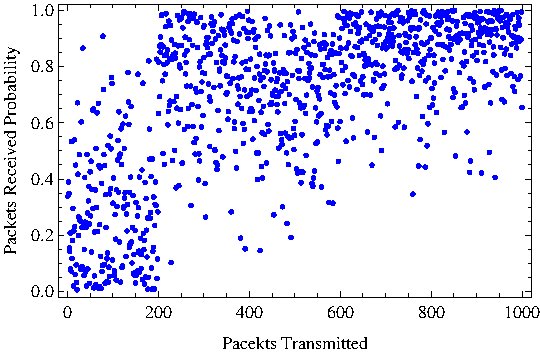
\includegraphics[width=5in]{chap3/mobile.pdf}
\bicaption[fig:mobile_k]{数据包接收成功概率}{数据包接收成功概率}{Fig}{Packets Received Probability}
\end{figure}

从式(\ref{equa:Eps})和式(\ref{equa:Dps})可以看出,DSWA的测量误差同样与$p_i$的变化情况有关,总体上相对于EWMA在移动网络条件下具有更高的精度与测试开销。如图 \ref{fig:mobile} 所示,当$p_i$同样设置为图 \ref{fig:mobile_k} 中情形时,DSWA以同样的窗口长度能够实现更频繁的采样,同时具有更高的测量精度,相对于EWMMA的0.19到0.32的测量误差,DSWA在$\beta=0.3$时能够将测量误差降低为0.001。

\begin{figure}[!htp]
\centering
\subfigure[Weighted Window Length $(\alpha=0.4)$]{
    \label{fig:weighted_m}
    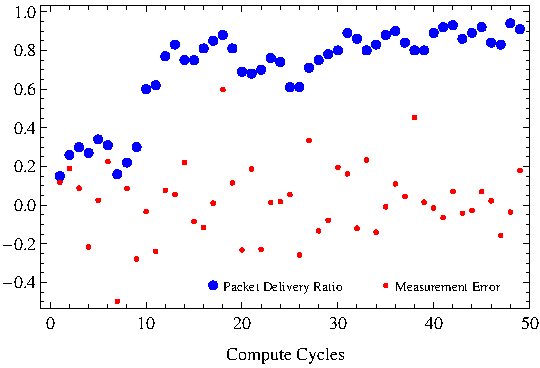
\includegraphics[width=2.5in]{chap3/weighted_m.pdf}}
    \hspace{1cm}
\subfigure[Sliding Window Length $(\beta=0.3)$]{
    \label{fig:sliding_m }
    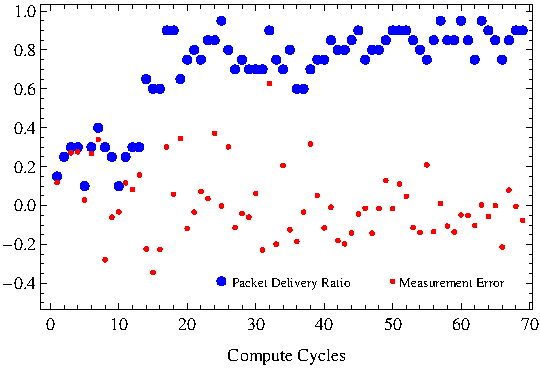
\includegraphics[width=2.5in]{chap3/sliding_m.pdf}}
\bicaption[fig:mobile]{移动网络测试精度}{移动网络测试精度}{Fig}{Measurement Window Length in Mobile Wireless Networks ($W=20$)}
\end{figure}

\begin{table}[!htp]
\renewcommand{\arraystretch}{1}
\bicaption[tab:footnote]{加权算法测试误差}{加权算法测试误差}{Table}{Measurement Error of Weighted Window Length}
  \centering
\begin{threeparttable}[b]
\label{error}
\begin{tabular}{c|ccccc}
\hline
$\pmb{\alpha}$ & 0.1   & 0.2   & 0.3   & 0.4   & 0.5 \\
\hline
$\textbf{E[}\Delta PDF_w\textbf{]}$  & 0.026 & 0.032 & 0.019 & 0.020 & 0.029 \\
$\textbf{D[}\Delta PDF_w\textbf{]}$  & 0.035 & 0.032 & 0.032 & 0.036 & 0.040 \\
\hline
\end{tabular}
\end{threeparttable}
\end{table}

\begin{table}[!htp]
\renewcommand{\arraystretch}{1}
\bicaption[tab:footnote]{滑动算法测试误差}{滑动算法测试误差}{Table}{Measurement Error of Sliding Window Length}
\centering
\begin{threeparttable}[b]
\label{error}
\begin{tabular}{c|ccccccccc}
\hline
$\pmb{\beta}$ & 0.1   & 0.2   & 0.3   & 0.4   & 0.5   & 0.6   & 0.7   & 0.8   & 0.9 \\
\hline
$\textbf{E[}\Delta PDF_s\textbf{]}$ & 0.040 & 0.003 & 0.001 & 0.010 & 0.015 & 0.013 & 0.008 & 0.021 & 0.007 \\
$\textbf{D[}\Delta PDF_s\textbf{]}$ & 0.036 & 0.037 & 0.038 & 0.029 & 0.039 & 0.038 & 0.029 & 0.038 & 0.036 \\
\hline
\end{tabular}
\end{threeparttable}
\end{table}

\begin{figure}[!htp]
\centering
\subfigure[a=1,b=3]{
    \label{fig:error1}
    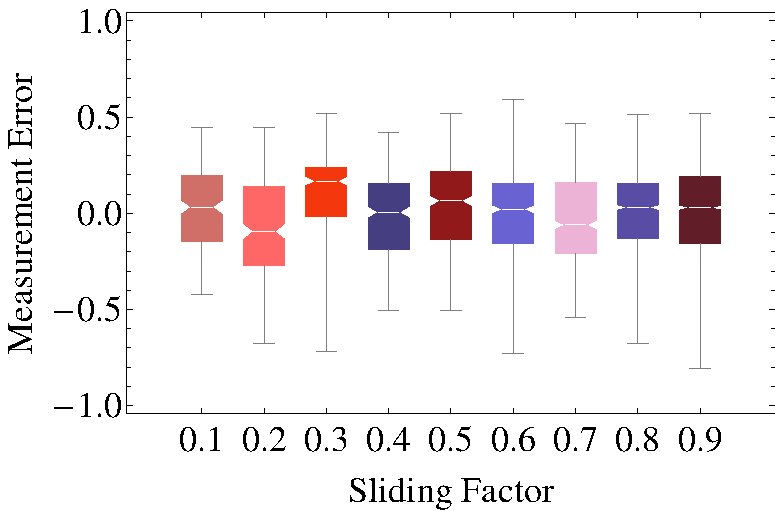
\includegraphics[width=2.5in]{chap3/error1.pdf}}
    \hspace{1cm}
\subfigure[a=3,b=1]{
    \label{fig:error2}
    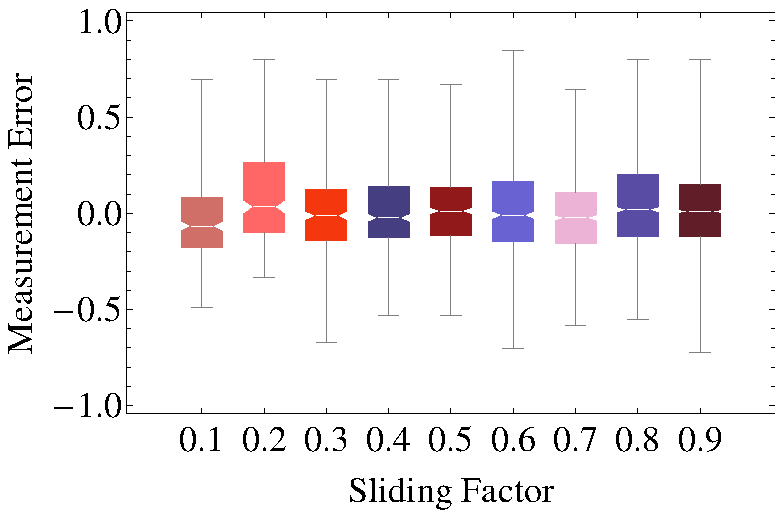
\includegraphics[width=2.5in]{chap3/error2.pdf}}
\hspace{1in}
\centering
\subfigure[a=5,b=2]{
    \label{fig:error3}
    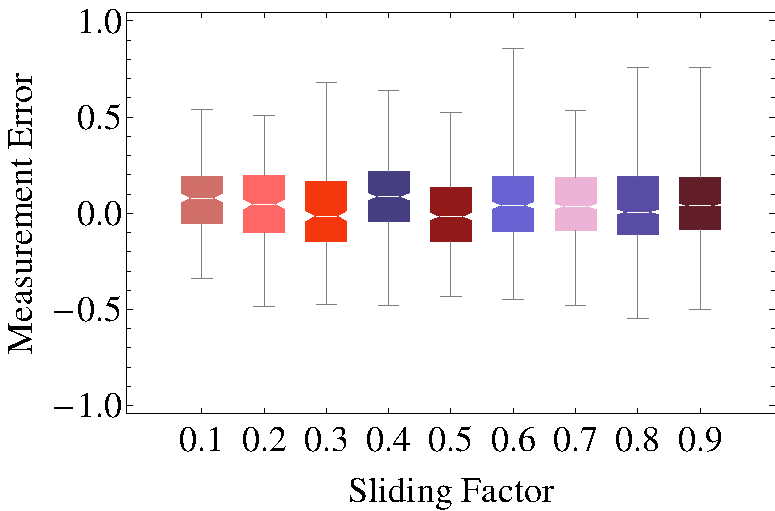
\includegraphics[width=2.5in]{chap3/error3.pdf}}
    \hspace{1cm}
\subfigure[a=5,b=1]{
    \label{fig:error4}
    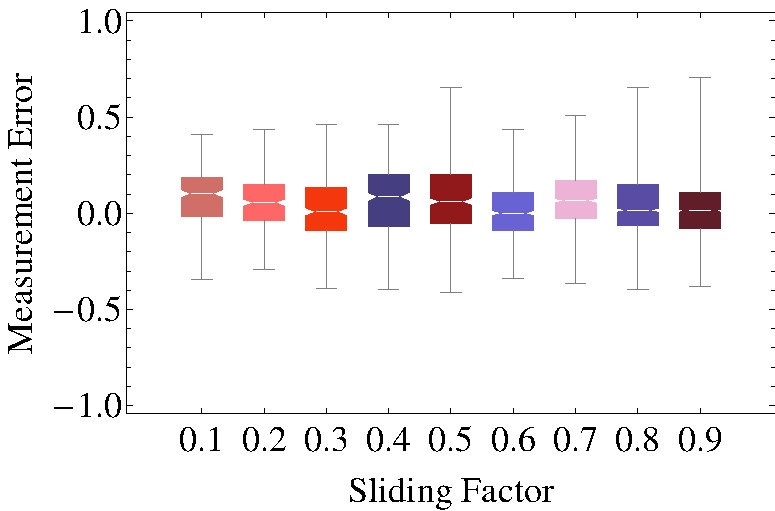
\includegraphics[width=2.5in]{chap3/error4.pdf}}
\bicaption[fig:mobile_e]{动态滑动平均测试精度}{动态滑动平均测试精度}{Fig}{Measurement Errors of Sliding Window Length Method}
\end{figure}
%
%\begin{figure}[!t]
%\centering
%  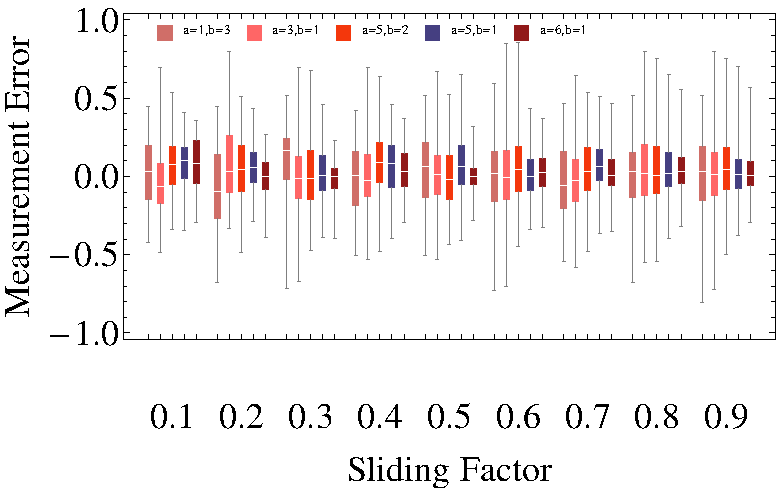
\includegraphics[width=0.5\textwidth]{error.pdf}
%\caption{Measurement Errors of Sliding Window Length Method}
%\label{mobile_e}
%\end{figure}

\section{链路质量在线建模}
\label{sec:modeling}

除了进行准确的PDR测量之外,还需要对链路层指标与物理层指标进行建模,即基于实测数据的PDR-RSS模型,并进行在线更新以提供准确的网络状态信息,从而为频谱分配及速率适配提供可靠输入。本文提出在线PDR-RSS建模框架,通过同时利用物理层及链路层信息,提高移动MIMO-OFDM网络信息的可靠传输与的速率的有效配置。在线PDR-RSS建模框架如图 \ref{fig:onlinemodel} 所示,该框架主要由三部分构成:
\begin{itemize}
  \item \textbf{PDR-RSS数据库:}PDR与RSS在不同MIMO-OFDM配置下的原始数据
  \item \textbf{PDR-RSS模型:}不同MIMO-OFDM配置下PDR-RSS模型过渡窗口上限
  \item \textbf{HT-GI-MCS索引:}MIMO-OFDM配置选择序列
\end{itemize}

\begin{figure}[!htp]
\centering
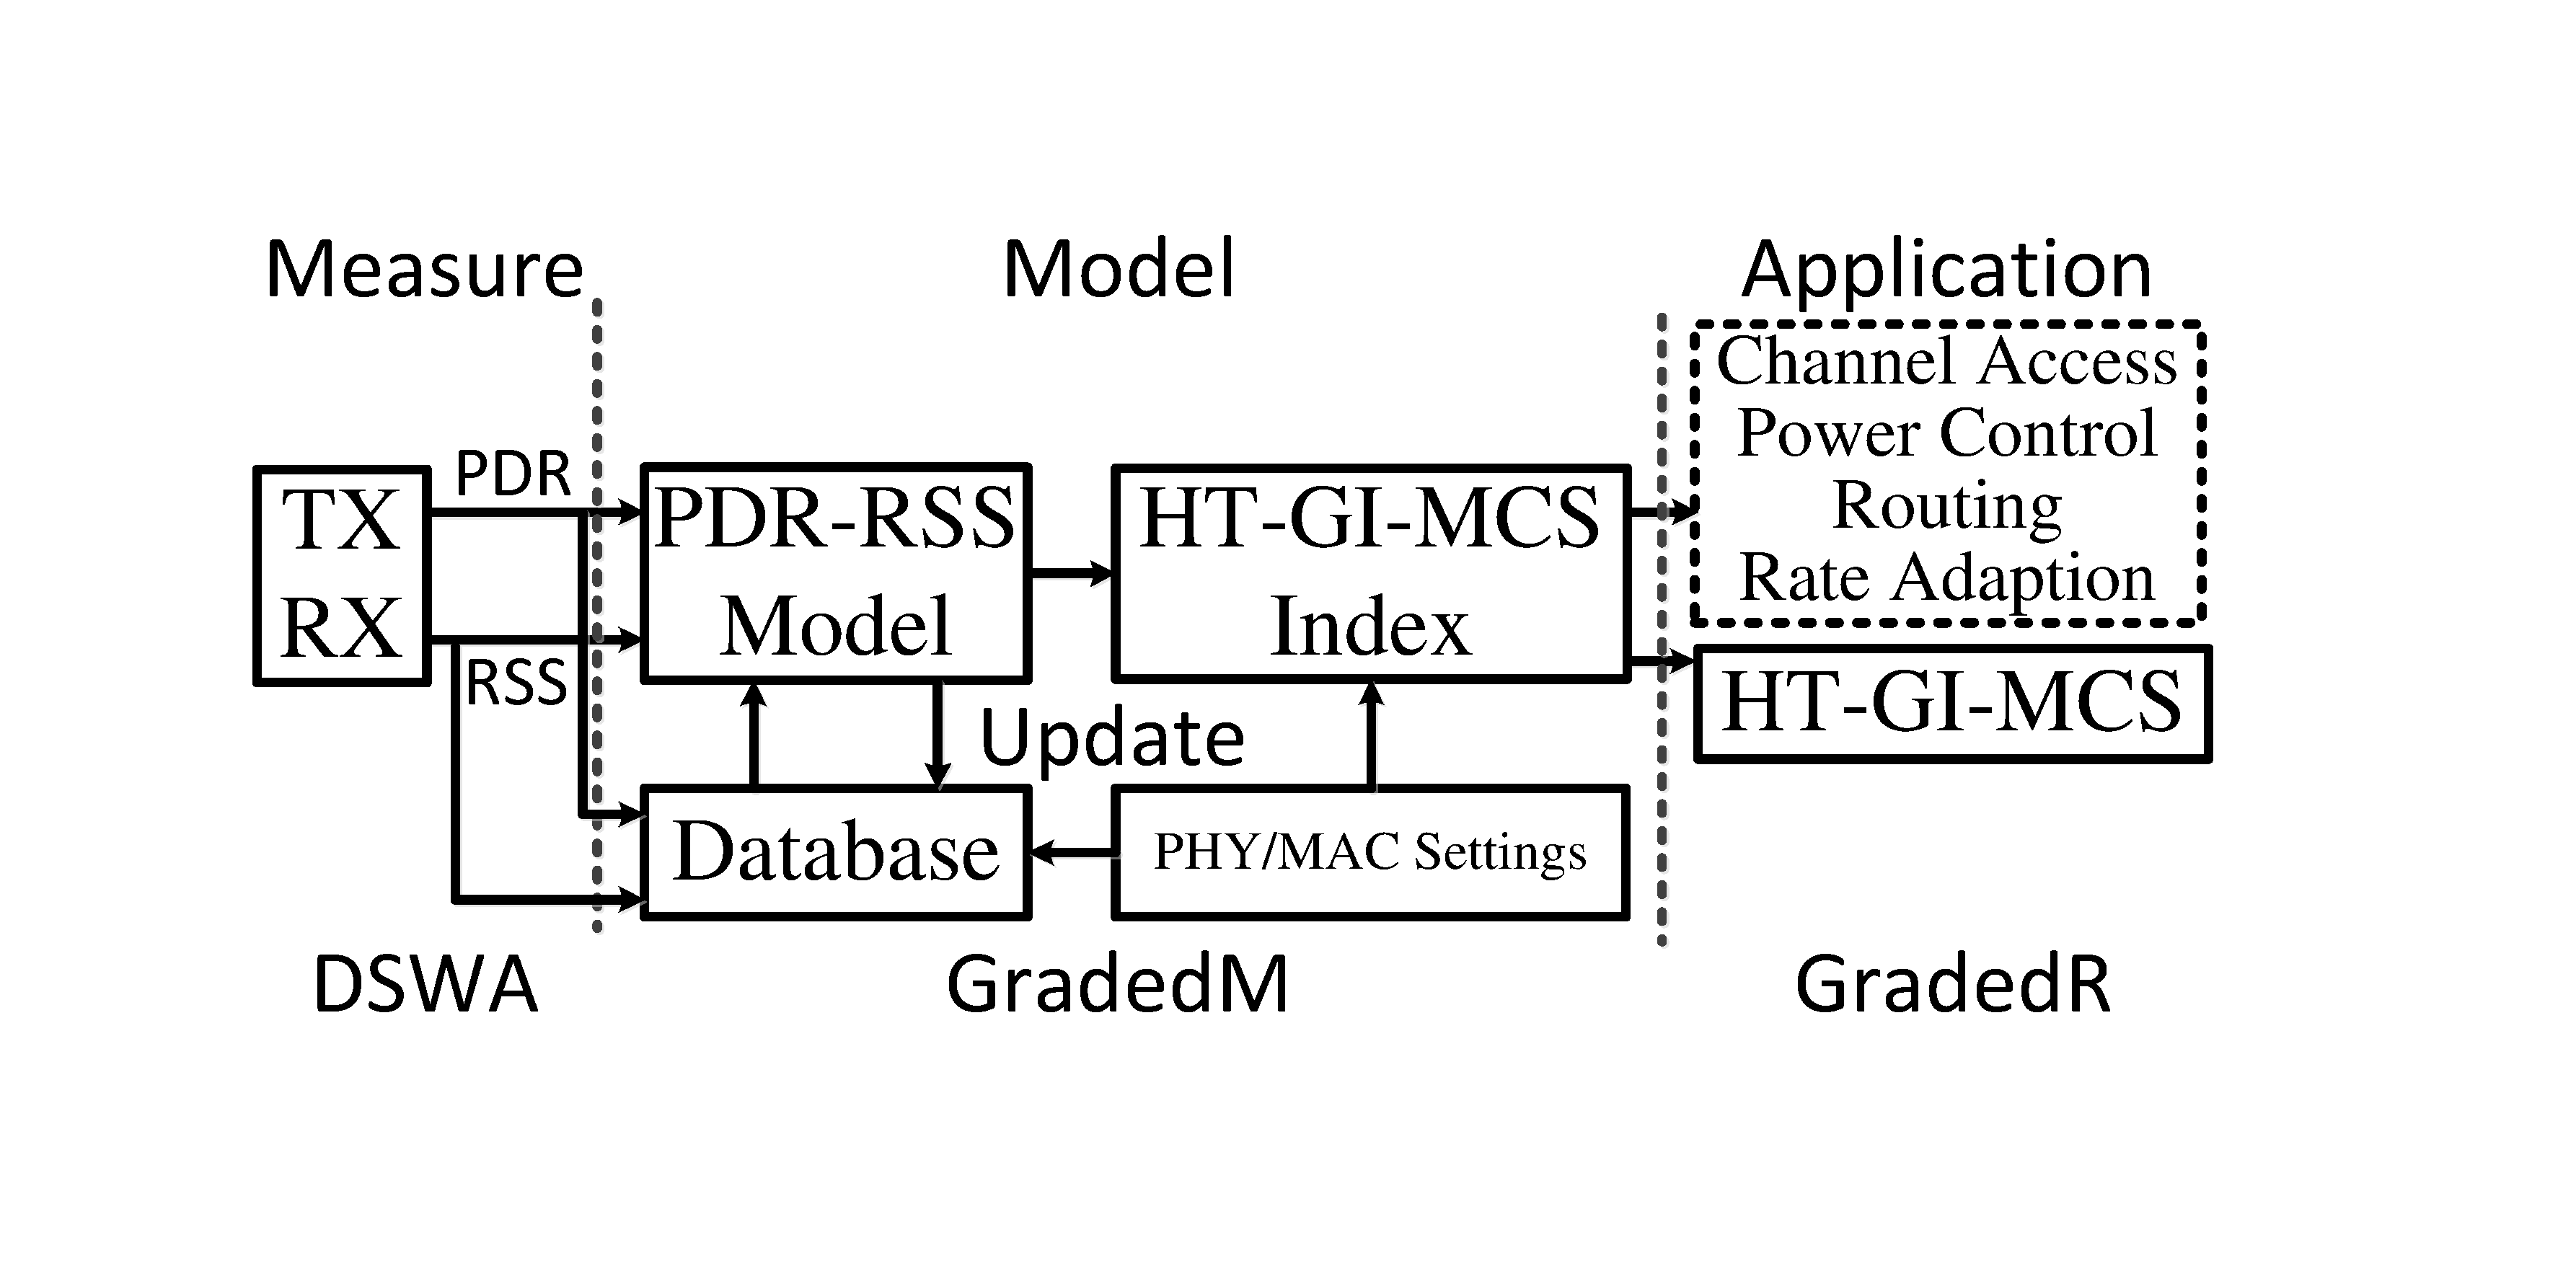
\includegraphics[width=0.8\textwidth]{chap3/modeling.pdf}
\bicaption[fig:onlinemodel]{动态PDR-RSS模型框架}{动态PDR-RSS模型框架}{Fig}{Dynamic PDR-RSS modeling framework}
\end{figure}

该框架主要由以下三步进行初始化与在线更新:
\begin{enumerate}
  \item 通过离线实验采集不同MIMO-OFDM配置下PDR及RSS的原始数据,建立PDR-RSS初始模型;
  \item 通过在线实测PDR及RSS数据对不同MIMO-OFDM配置下的PDR-RSS模型进行在线更新;
  \item 通过当前PDR及RSS相对与不同MIMO-OFDM配置下PDR-RSS模型过渡窗口上限的差值,形成MIMO-OFDM配置选择序列。
\end{enumerate}

通过以上的在线PDR-RSS建模过程,该建模框架相对于传统的静态PDR-RSS模型框架(图 \ref{fig:offlinemodel})具有明显的优点。第一,在线PDR-RSS 建模框架中数据库与PDR-RSS模型同时具有两个输入变量,而不是单独利用PDR或RSS;第二,在线框架中PDR-RSS模型和数据库同时进行在线更新,而不是只对PDR进行更新,或利用静态PDR-RSS模型而只对RSS进行更新;第三,在线框架根据当前PDR和RSS信息与模型,实时更新能够实现可靠通信的MIMO-OFDM 配置序列,并对其按照可获得性能进行排序,而不是随机探测某一配置。因此在线PDR-RSS建模框架针对静态PDR-RSS框架在信道状态和链路质量信息方面,提供了系统化的解决方案,在保证移动MIMO-OFDM网络可靠通信的前提下\footnote{在系统运行过程中保证$PDR>P_{thrh}=90\%$且$RSS>\delta_+=GradedT(HT, GI, MCS)$},提供最优的MIMO-OFDM配置选择序列。


\subsection{模型初始化}
\label{sec:initial}

802.11n标准采用多种物理层及链路层技术,实现更高的吞吐量和更广的覆盖范围。在物理层,802.11n网络利用MIMO技术实现空间复用与分集,同时利用OFDM调制方式以降低信号干扰并提升频谱利用效率,802.11n网络利用信道绑定技术可以将相邻两个20MHz的信道作为一个40MHz信道使用,从而有效提升网络吞吐量;在链路层,802.11n网络使用短保护间隔(Short Guard Interval, SGI)及帧聚合技术,以降低通信开销并提高传输效率。802.11n 网络通过以上的物理层与链路层技术,一方面能够有效提升网络性能,另一方面提高了信道状态估计和链路质量测试的复杂度,对于不同的MIMO-OFDM 配置,PDR-RSS模型具有不同特点。

为了实现802.11n网络的在线PDR-RSS建模框架,本文首先通过大量实验数据对PDR-RSS模型进行刻画,以及该模型与物理层和链路层配置的关系,主要包括信道带宽HT、调制与编码策略MCS和保护间隔长度GI。其中信道带宽分为HT=\{HT20, HT40\},保护间隔长度类型分为GI=\{LGI, SGI\},MCS与MIMO 配置有关,对于3$\times$3的MIMO系统而言,MCS=\{0, 1, 2, ..., 23\}。除了网络配置之外,还需要对网络的不同位置与路线进行刻画,对802.11n 网络的PDR-RSS 模型的刻画至少需要500次重复实验,以完整包括网络的不同配置与网络状态,以下为通过这些实验数据对802.11n网络的PDR-RSS模型的总结。

\begin{figure}[!htp]
\centering
    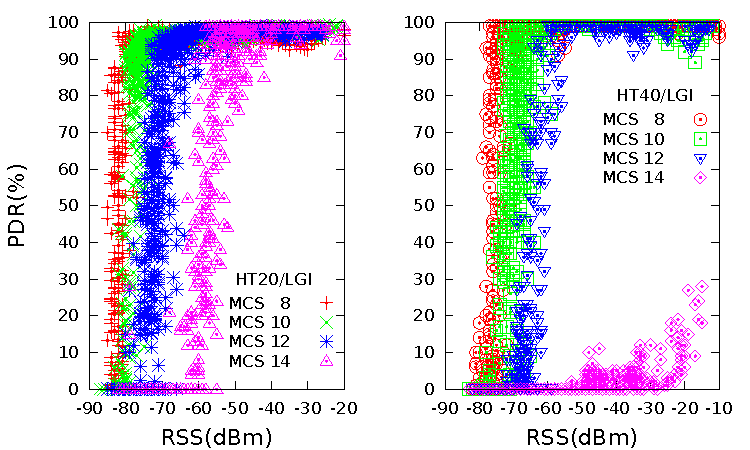
\includegraphics[width=4in]{chap3/pdr_ch_lgi.pdf}
\bicaption[fig:pdr_lgi]{链路质量模型,HT=HT20/HT40,MCS=8-14,GI=LGI}{链路质量模型,HT=HT20/HT40,MCS=8-14,GI=LGI}{Fig}{PDR-RSS model of HT=HT20/HT40, MCS=8-14, GI=LGI}
\end{figure}

\begin{figure}[!htp]
\centering
    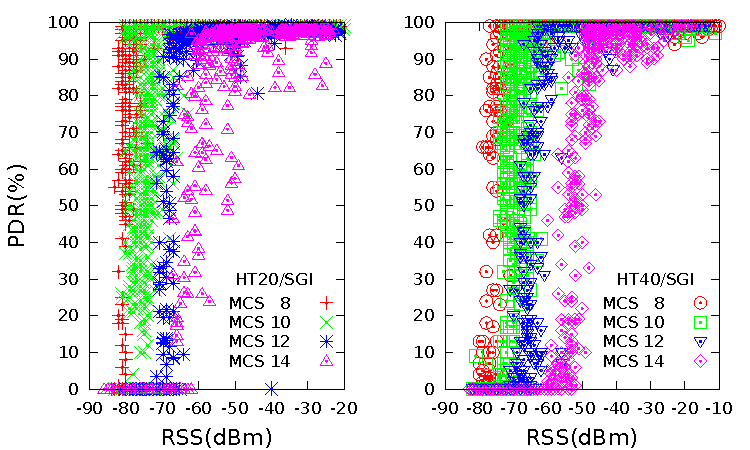
\includegraphics[width=4in]{chap3/pdr_ch_sgi.pdf}
\bicaption[fig:pdr_sgi]{链路质量模型,HT=HT20/HT40,MCS=8-14,GI=SGI}{链路质量模型,HT=HT20/HT40,MCS=8-14,GI=SGI}{Fig}{PDR-RSS model of HT=HT20/HT40, MCS=8-14, GI=SGI}
\end{figure}

\begin{enumerate}
  \item \textbf{信道带宽:}
  802.11n网络中定义了HT20与HT40两种信道带宽,其中HT40信道能够实现单位信号流高达150Mbps的传输速率,当链路质量能够得到有效保证时,可以获得20MHz 信道传输速率的两倍以上。但是另一方面HT40信道更容易受到信号干扰的影响,从图 \ref{fig:pdr_lgi} 可以看出,在不同的调制与编码策略及保护间隔情形下,HT40 信道的接收灵敏度明显高于HT20信道。同时可以看出HT40与HT20信道的过渡窗口长度基本相同,当MCS从8增加到14,HT20/HT40信道的过渡窗口长度从3dB变化为10dB。另一方面在适中的数据传输速率范围内,HT40信道能够在相同的传输速率基础上提供更广的覆盖范围。
  \item \textbf{调制编码:}
  不同的调制与编码策略对于802.11n网络的PDR-RSS模型具有很大影响,图 \ref{fig:pdr_lgi} 与图 \ref{fig:pdr_sgi} 刻画了在HT=HT20/HT40和GI=LGI/SGI 下PDR-RSS模型与MCS的关系。第一,接收灵敏度随着MCS的上升而增大,当MCS从8增加到14时,HT20/SGI与HT40/SGI的接收灵敏度分别在(-80dBm, -50dBm)和(-80dBm, -40dBm)范围内递增;第二,过渡窗口长度$\rho$同样随着MCS的上升而增大,尤其当传输速率高于115Mbps时,从图 \ref{fig:pdr_sgi} 中可以看出,当MCS=12时$\rho$甚至达到15dB,而过长的过渡窗口长度会严重降低网络的有效吞吐量。
  \item \textbf{保护间隔:}
  802.11n网络采用短保护间隔以进一步提升网络性能,理论上GI=SGI可以获得11\%的传输速率的提升 \upcite{perahia2008next}。当传输速率较低时,SGI与LGI 的传输成功率和吞吐量没有很大分别,如图 \ref{fig:pdr_lgi} 和图 \ref{fig:pdr_sgi} 所示。但是当传输速率较高时,SGI可以明显提高网络性能,尤其对于HT40信道而言,如图 \ref{fig:pdr_sgi_high} 所示,对于HT=HT40且MCS=15时,LGI的PDR总是低于40\%,而对于HT20与HT40信道,SGI的PDR分别可以得到10\%-40\%和20\%-60\%提升。
\end{enumerate}

\begin{figure}[!htp]
\centering
    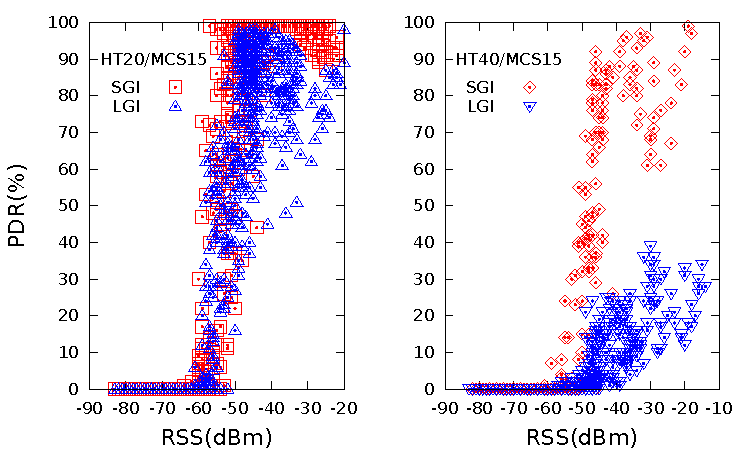
\includegraphics[width=4in]{chap3/pdr_sgi.pdf}
\bicaption[fig:pdr_sgi_high]{链路质量模型,HT=HT20/HT40,MCS=15,GI=LGI/SGI}{链路质量模型,HT=HT20/HT40,MCS=15,GI=LGI/SGI}{Fig}{PDR-RSS model of HT=HT20/HT40, MCS=15, GI=LGI/SGI}
\end{figure}

通过以上的PDR-RSS模型初始化与性质刻画,可以得到PDR-RSS的初始模型,即在不同MIMO-OFDM配置下PDR-RSS过渡窗口参数。在系统实现时定义为结构体GradedT,该结构体的初始参数可以通过复杂度为$\textit{O}(N \cdot w \cdot g \cdot r)$的实验得到,其中$N$为测试通信节点数目,$w$为某特定中心频率下的信道带宽类型, $g$为保护间隔类型,$r$为调制与编码策略数目。对于具有3$\times$3MIMO配置的802.11n系统,$w=4$代表在中心频率2.4GHz 及5GHz下分别具有HT20与HT40两种信道类型,$g=2$表示LGI和SGI两种保护间隔类型,$r=24$对应于0-23的调制与编码索引。

\begin{figure}[!htp]
\centering
    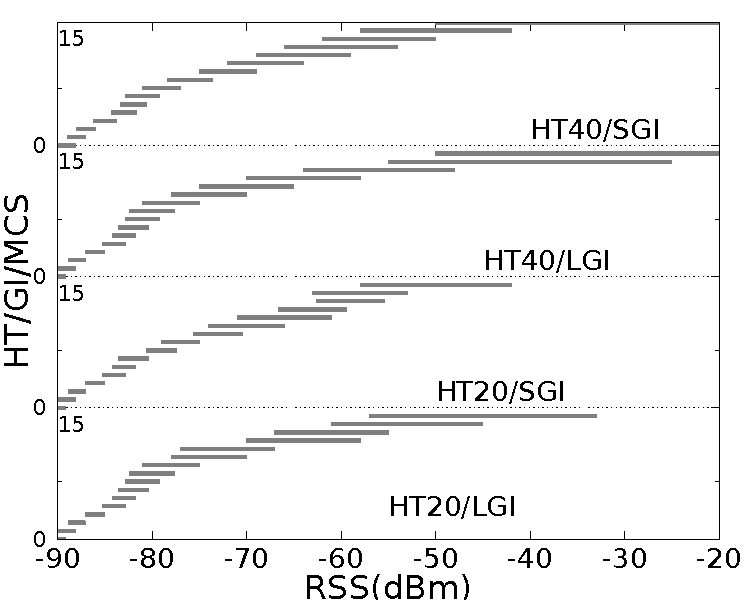
\includegraphics[width=0.8\textwidth]{chap3/graded.pdf}
\bicaption[fig:modelbegin]{PDR-RSS初始模型}{PDR-RSS初始模型}{Fig}{Initial PDR-RSS model}
\end{figure}

该PDR-RSS初始模型在系统运行时进行在线更新,2$\times$2MIMO系统的GradedT如图 \ref{fig:modelbegin} 所示,GradedT将HT/GI/MCS选择序列划分为三个区域,如果某一配置刚好位于灰色分界线的右边,则意味着该配置在当前网络状态下可以保证信号的可靠传输\footnote{即在此配置下当前RSS可以保证PDR>$P_{thrh}$=90\%},因此在当前RSS条件下所有位于灰色分界线右边的配置中,可以选择最优的配置以提高网络吞吐量。

\subsection{模型在线更新}
\label{sec:update}

在线PDR-RSS建模主要实现PDR-RSS模型与数据库的实时更新,并根据当前网络状态生成HT/GI/MCS配置选择序列,本文将这一过程简称为GradedM。首先,当RSS 或PDR其中任何某一指标低于设置的门限值时,GradedM便对PDR-RSS模型进行更新。显然,MIMO-OFDM网络某一配置在当前状态下可以获得的可靠性,可以由每一配置下PDR-RSS模型过渡窗口上限$\delta_+$ 与当前接收信号强度RSS 的距离表示,即RSS-GradedT。据此可以根据当前RSS与GradedT 进行MIMO-OFDM 配置排序,从而生成HT/GI/MCS 选择序列。以上过程的伪代码如算法 \ref{alg:graded} 所示。

\begin{algorithm}[!htp]
\floatname{algorithm}{算法}
\renewcommand{\algorithmicrequire}{\textbf{输入:}}
\renewcommand{\algorithmicensure}{\textbf{输出:}}
\caption{GradedM:PDR-RSS在线建模与实时更新}
\label{alg:graded}
\begin{algorithmic}[1]
\Require pdr-now, rss-now
\Ensure  ht-gi-mcs-index
\State{\label{graded-table}struct GradedT \{ \\ ~~~~~~~~~graded-delta[r][2]; // r=8/16/24 对应于天线数量1/2/3\\ \} graded-table[w][g]; // w=g=2 对应于信道HT20/HT40与保护间隔LGI/SGI\label{graded-table2}}
\State{// 1. PDR-RSS模型实时更新}
\If{graded-delta-changed} \label{delta-changed}
\State{graded-table $\gets$ update-delta(pdr-now,rss-now);}
\EndIf \label{delta-updated}
\State{// 2. HT/GI选择序列排序}
\State{mcs-index $\gets$ sort(graded-table,rss-now);} \label{ht-gi}
\State{// 3. HT/GI/MCS选择序列排序}
\State{ht-gi-mcs-index $\gets$ sort(mcs-index,mcs-rate);} \label{ht-gi-mcs}
\State \Return{ht-gi-mcs-index;}
\end{algorithmic}
\end{algorithm}

在算法 \ref{alg:graded} 中,结构体GradedT(第 \ref{graded-table} 行到第 \ref{graded-table2} 行)定义了不同MIMO-OFDM配置PDR-RSS模型过渡窗口的上下限值,通过当前的PDR和RSS可以对此上下限的变化进行判断,如果某一门限值发生了变化则进行实时更新 (第 \ref{delta-changed} 行到第 \ref{delta-updated} 行)。对于所有位于过渡窗口上限右边的配置,GradedM首先根据当前RSS与过渡窗口上限的差值\footnote{即RSS-$\delta_+$=RSS-GradedT(HT, GI, MCS),单位为dB},对所有可靠配置排序生成HT/GI选择序列(第 \ref{ht-gi} 行),从而得到当前可选择配置序列;但此时可选序列并未按照所能获得吞吐量进行排序,然后GradedM根据可获得的传输速率与HT/GI选择序列,排序得到HT/GI/MCS选择序列(第 \ref{ht-gi-mcs} 行),此时的HT/GI/MCS序列可以保证可靠数据传输,并按照可获得的网络吞吐量排序。由GradedM所产生的HT/GI/MCS选择序列通过网络可靠性、数据传输速率以及当前网络状态产生,因此可以通过修改或直接应用于其他上层应用中。

综上所述,802.11n网络在线PDR-RSS建模框架主要由三部分构成:信道状态估计与链路质量测试、PDR-RSS初始模型与数据库的形成以及PDR-RSS模型在线更新与配置排序。通过在线建模框架能够实现MIMO-OFDM系统的物理层与链路层的有效配置,实现网络可靠性、数据传输速率的有效平衡,在保证系统可靠性的前提之下有效提高网络吞吐量。

\section{系统实现}
\label{sec:system_link}

本章主要介绍在线建模框架的系统实现,主要包括测试平台开发与搭建和算法设计与实现,其中包括速率控制算法的设计与实现,以实现对在线建模框架性能的有效评估。

\subsection{实验平台}
\label{sec:platform80211n}

802.11n网络测试平台主要由无线接入点(Access Point, AP)、静态节点及移动节点组成,其中AP为TP-LINK的双频无线路由器TL-WRD4310,其无线通信芯片为Atheros AR9580无线模块,该模块支持最高3$\times$3的MIMO配置,在HT20/HT40信道下能够实现300Mbps/450Mbps的无线数据传输速率,静态节点和移动节点分别为台式机和便携式笔记本,并配置Atheros的3天线双频无线网卡AR9380,所有的无线通信节点运行于Linux系统(内核版本 3.2.0-26),并通过\texttt{ath9k} \upcite{ath9k}开源无线驱动实现无线通信。

\begin{figure}[!htp]
\centering

\includegraphics[width=0.9\textwidth]{chap3/testbed.pdf}
\bicaption[fig:testbed80211n]{802.11n网络测试系统}{802.11n网络测试系统}{Fig}{Experiment testbed and measurement setup for 802.11n networks}
\end{figure}

802.11n网络测试场景如图 \ref{fig:testbed80211n} 所示,包括宿舍与实验室两个室内环境,两者都包括LOS和NLOS信号传输,同时包含静态测试(\textbf{P1} 到 \textbf{P11})与移动测试(\textbf{r1} 到 \textbf{r6}),其中静态测试主要完成初始PDR-RSS模型刻画并形成模型数据库,移动测试实现在线建模框架及速率控制算法的评估。

\subsection{测试方法}
\label{sec:measurement80211n}

为了避免其他信号的干扰,所有实验运行在5.745GHz频段149信道,同时所有实验在0:00到6:00间进行。在静态与移动测试中,系统通过\texttt{iperf}\footnote{\url{http://iperf.sourceforge.net}} 周期性发送UDP数据包,数据包长度固定为1500bytes。实验测试过程中取消MAC层的RTS/CTS及ACK 机制,同时关闭功率节省模式,以降低其他因素的影响。静态实验通过不同位置的通信节点进行数据采集,完成不同MIMO-OFDM配置的初始建模,移动测试通过常速前进的移动节点进行测试,如图 \ref{fig:testbed80211n} 所示,以上实验可以完整覆盖移动MIMO-OFDM系统的所有配置与特性,从而完成对移动802.11n网络的测试与性能评估。

\subsection{速率控制}
\label{sec:adaption80211n}

根据在线建模框架,本文提出阶梯式速率控制算法GradedR,首先GradedR利用DSWA算法提高PDR测试精度并有效降低测试开销,然后通过在线建模实时更新PDR-RSS 模型并排序生成MIMO-OFDM配置选择序列,最后根据当前PDR和RSS在配置选择序列中确定最优配置。该速率控制算法的伪代码如算法 \ref{alg:pdr} 所示,其中PDR 的门限值设置为\{$P_{thrl},P_{thrh}$\}=\{$10\%,90\%$\},配置切换上下门限值分别设置为\{3dB, 10dB\}。

\begin{algorithm}[!htp]
\floatname{algorithm}{算法}
\renewcommand{\algorithmicrequire}{\textbf{输入:}}
\renewcommand{\algorithmicensure}{\textbf{输出:}}
\caption{GradedM $\rightarrow$ DSWA $\rightarrow$ GradedR}
\label{alg:pdr}
\begin{algorithmic}[1]
\Require tx-complete (packets transmitted event)
\Ensure  rate-index (rate selection indexes of HT/GI/MCS)
\State{// DSWA(pdr-last, pdr-now):更新加权平均中间变量$\gamma$和$\eta$,返回平均窗口长度$W$和滑动因子$\beta$}
\State{// GradedM(pdr, rss):更新PDR-RSS模型graded-table并对MIMO-OFDM配置进行排序,返回HT/GI/MCS选择序列ht-gi-mcs-index}
\State{// GradedR(ht-gi-mcs-index):保证当前网络PDR高于90\%,返回当前状态下的最优MIMO-OFDM配置ht-gi-mcs}
\If{pdr-now $<P_{thrh} |$ rss-now $<\delta_+ + low-limit-to-gray$} \label{alg:lowlimit}
\State{graded-talbe $\gets$ GradedM(pdr-now,rss-now);} // rc.c
\State{rate-index $\gets$ down-rate-mcs(ht-gi-mcs-table);}
\EndIf
\If{graded-sens - rss-now $>$ high-limit-to-gray} \label{alg:highlimit}
\State{rate-index $\gets$ up-rate-mcs(ht-gi-mcs-table);}
\EndIf
\State \Return{\{tx-status,rate-index\};}
\end{algorithmic}
\end{algorithm}

如果当前配置下过渡窗口上限与当前RSS之差低于3dB时或高于10dB时,系统将根据HT/GI/MCS选择序列进行重新配置。如果该距离低于3dB(第 \ref{alg:lowlimit} 行),则在当前HT/GI选择区域内选择更低的MCS 配置以降低传输速率,或在其他HT/GI区域内选择相同的MCS配置以保证当前传输速率;相反当此距离大于10dB时(第 \ref{alg:highlimit} 行),GradedR将提高MCS 以提升网络性能,同样优先在当前HT/GI 区域内进行选择。考虑到在第\ref{sec:initial}节中关于保护间隔对PDR-RSS模型的影响,在配置选择过程将SGI作为最后选择,即当且仅当在LGI配置下的最高MCS仍然无法满足PDR或传输速率要求时,则选择SGI配置以保证网络性能。

\begin{figure}[!htp]
\centering
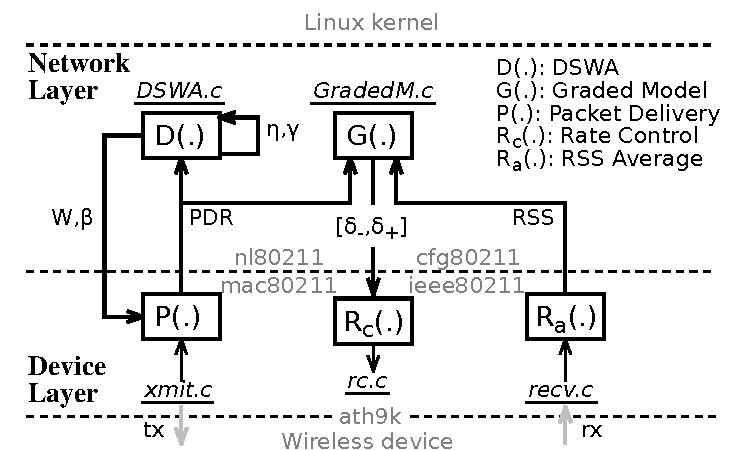
\includegraphics[width=5in]{chap3/framework.pdf}
\bicaption[fig:gradedframework]{链路质量测试算法}{链路质量测试算法}{Fig}{Measurement framework and implementation on Linux systems}
\end{figure}

以上速率控制算法通过\texttt{ath9k} 开源无线驱动运行于Linux操作系统之上,图 \ref{fig:gradedframework} 为802.11n网络性能测试与速率控制的软件框架,主要由驱动层和网络层两部分构成。网络层进行DSWA参数计算以确定平均窗口长度和滑动因子,同时通过GradedT对配置选择序列进行实时更新;驱动层由数据包发送和接收事件驱动,负责执行PDR计算和RSS平均,同时根据当前PDR和RSS结果结合网络层的配置选择序列,进行重新配置的判断与执行。

\section{性能评估}
\label{sec:evaluation80211n}

性能评估部分包括测试精度与开销的对比以及系统的吞吐量评估,本章首先对DSWA和EWMA测试算法的测试精度与开销进行了对比,然后详细分析评估了DSWA和在线PDR-RSS建模框架对系统性能的提升。

\subsection{传输成功率}
\label{sec:pdr}

在静态无线网络中,接收信号强度在短时间内基本保持不变 \upcite{reis2006model},可以认为在PDR测试过程中$p_i$恒定不变,则$x_i$为独立同分布随机变量,此时可以刻画为伯努利过程,即$\textbf{P(}x_i=1\textbf{)}=p$且$X\sim B(p)$,此时DSWA和EWMA都是被测PDR的无偏估计,因此具有相同的测试精度,而DSWA可以有效降低测试开销。但是在实际网络中,EWMA的测试精度明显低于DSWA,主要原因是$p_i$的时变特性,而在移动网络中还需要考虑网络的空间特性。图 \ref{fig:DSWA_error} 为移动网络中EWMA和DSWA算法测试误差的累积分布函数(Cumulative Distribution Function, CDF),对于DSWA测试算法而言,其测试误差在$\pm$0.008之间,而EWMA的测试误差为-0.019到0.032。同时从EWMA算法测试误差的CDF曲线可以看出,其测试误差相对于$Error=0$整体右移,说明EWMA算法的PDR测试结果相对于真实值普遍偏高,从而影响网络性能。相对于EWMA测试算法,DSWA算法在整体的测试精度上可以提高89\%。

\begin{figure}[!htp]
\centering
    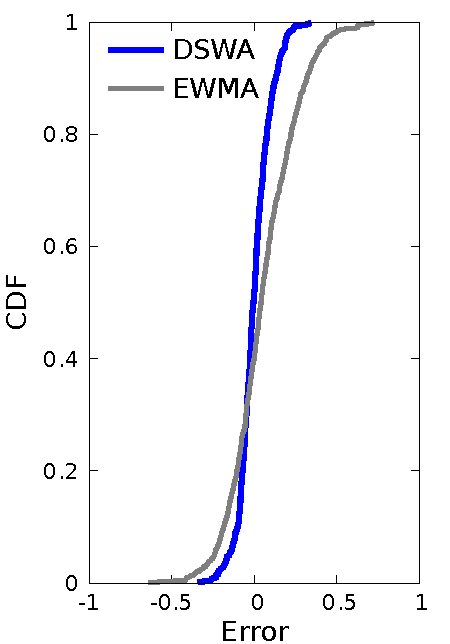
\includegraphics[width=2in]{chap3/cdf.pdf}
\bicaption[fig:DSWA_error]{传输成功率测试精度}{传输成功率测试精度}{Fig}{Measurement accuracy for EWMA and DSWA}
\end{figure}

除了能够提升移动802.11n网络PDR的测试精度之外,DSWA同时可以有效降低PDR的测试开销。首先DSWA的采样间隔$W$为前$n$次采样结果的加权平均,因此可以避免信号噪声引起的突变,同时对于PDR的变化作出快速反应;同时由于采样间隔$W$与PDR的相对变化密切相关,因此可以在链路质量持续下降时作出及时反应,并在网络状态保持稳定是降低采样频率。图 \ref{fig:DSWA_overhead} 给出DSWA在不同网络状态下的PDR测试开销,首先PDR在约15s时开始降低,采样间隔$W$和滑动因子$\beta$ 相应地降低;当PDR从40s到50s逐渐上升并趋于稳定时,采样间隔$W$从100逐渐增加为200,从而明显降低测试开销。而对于EWMA测试算法而言,其采样间隔在特定传输速率下基本保持不变,比如在传输速率为6.5Mbps时采样间隔为$W=20$,而在300Mbps时采样间隔上升为$W=500$。

\begin{figure}[!htp]
\centering
    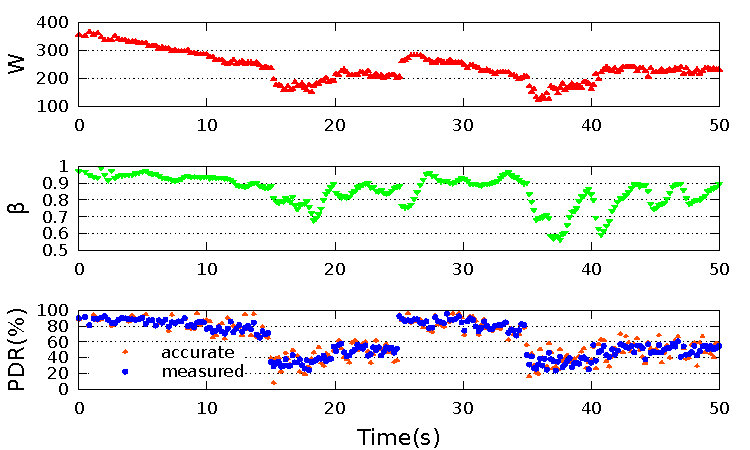
\includegraphics[width=5in]{chap3/DSWA.pdf}
\bicaption[fig:DSWA_overhead]{传输成功率测试开销}{传输成功率测试开销}{Fig}{Measurement overhead for EWMA and DSWA}
\end{figure}

\subsection{吞吐量}
\label{sec:throughput}

为了进一步对在线PDR-RSS建模框架和速率控制算法GradedR进行性能评估,本文通过便携式笔记本进行移动测试,所有的移动节点通过Linux操作系统和\texttt{ath9k} 开源无线驱动实现无线通信,并安装GradedR算法实现网络性能测试与速率控制,物理层的吞吐量作为性能评估指标。首先通过简单的移动测试,对速率控制算法在特定移动路线的稳定性与可靠性进行评估;然后在不同移动路线进行大量移动实验,分析在不同速率控制算法下吞吐量与平均RSS 的关系,通过统计分析分别分析DSWA测试算法及GradedR速率控制算法的性能提升情况。以上所有实验分别在1$\times$3、2$\times$3和3$\times$3的MIMO-OFDM系统下进行重复测试,以全面有效地对DSWA测试算法和GradedR速率控制算法进行性能评估。以下首先分析特定移动路线下的PDR和吞吐量关系,然后对所有移动路线的整体吞吐量与平均RSS的关系进行评估。

%\begin{figure}[!htp]
%\centering
%\begin{minipage}{2.5in}
%  \subfigure[1x3]{
%  \label{fig:route1}
%  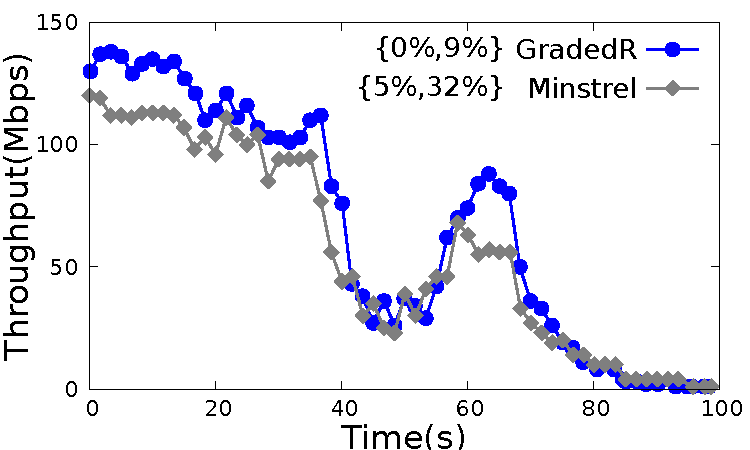
\includegraphics[width=2.5in]{chap3/route1.pdf}}
%  \hspace{1in}
%\centering
%  \subfigure[2x3]{
%  \label{fig:route2}
%  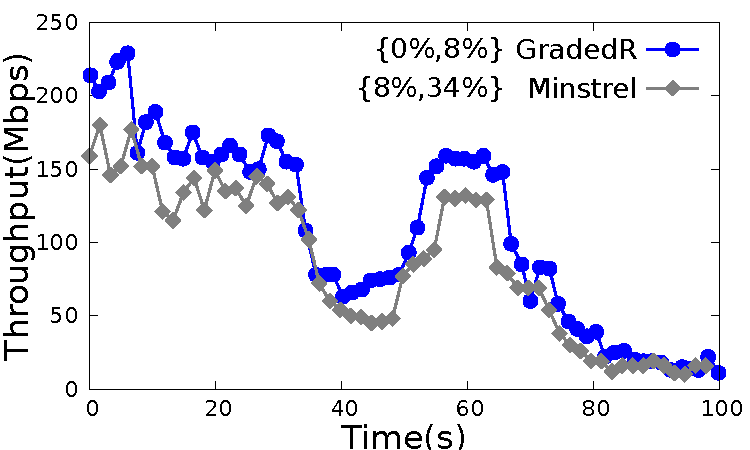
\includegraphics[width=2.5in]{chap3/route2.pdf}}
%  \hspace{1in}
%\centering
%  \subfigure[3x3]{
%  \label{fig:route3}
%  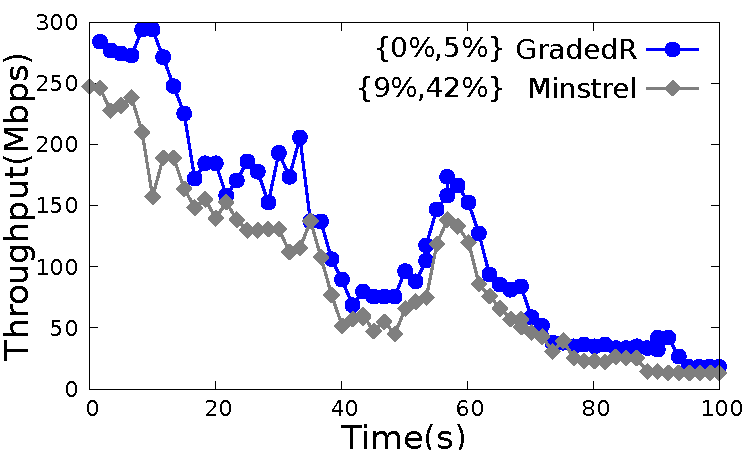
\includegraphics[width=2.5in]{chap3/route3.pdf}}
%\end{minipage}
%\begin{minipage}{2.5in}
%  \subfigure[1x3]{
%  \label{fig:thruput1}
%  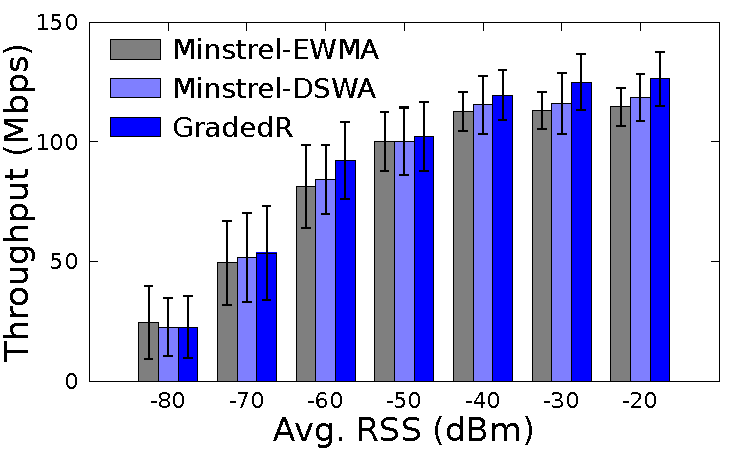
\includegraphics[width=2.5in]{chap3/goodput1.pdf}}
%  \hspace{1in}
%\centering
%  \subfigure[2x3]{
%  \label{fig:thruput2}
%  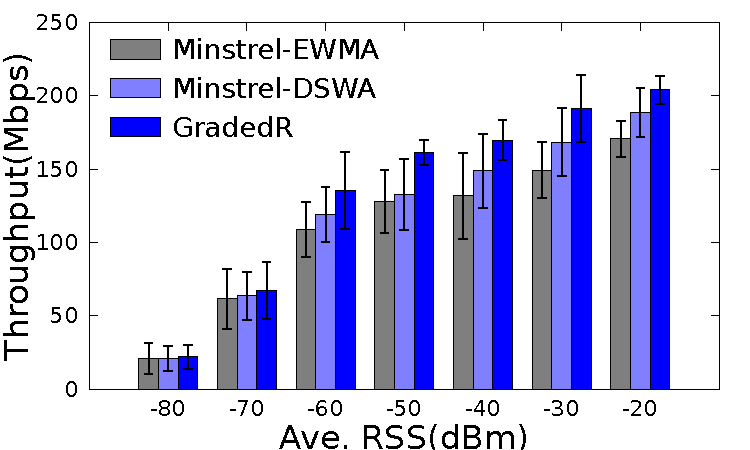
\includegraphics[width=2.5in]{chap3/goodput2.pdf}}
%  \hspace{1in}
%\centering
%  \subfigure[3x3]{
%  \label{fig:thruput3}
%  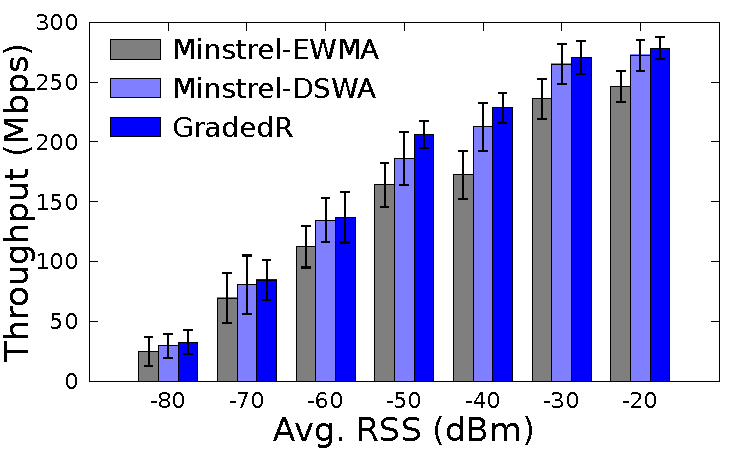
\includegraphics[width=2.5in]{chap3/goodput3.pdf}}
%\end{minipage}
%\bicaption[fig:route]{吞吐量、传输成功率与接收信号强度关系}{吞吐量、传输成功率与接收信号强度关系}{Fig}{Throughput improvements, PDR and RSS results along the route \textbf{r5}}
%\end{figure}

\begin{figure}[!htp]
\centering
  \subfigure[1x3]{
  \label{fig:route1}
  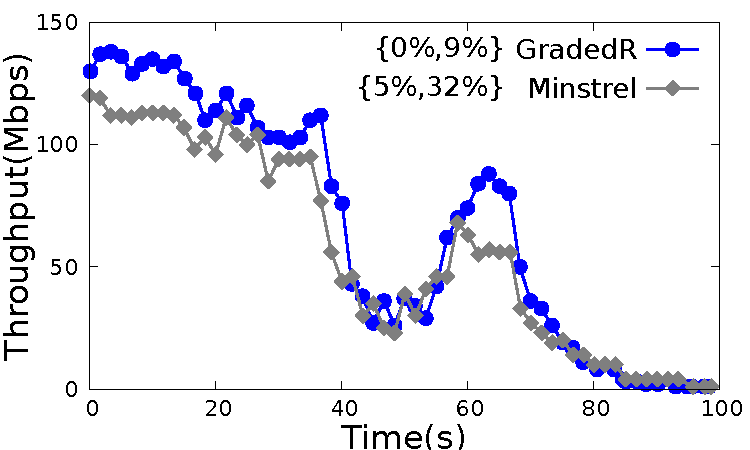
\includegraphics[width=3.6in]{chap3/route1.pdf}}
  \hspace{1in}
\centering
  \subfigure[2x3]{
  \label{fig:route2}
  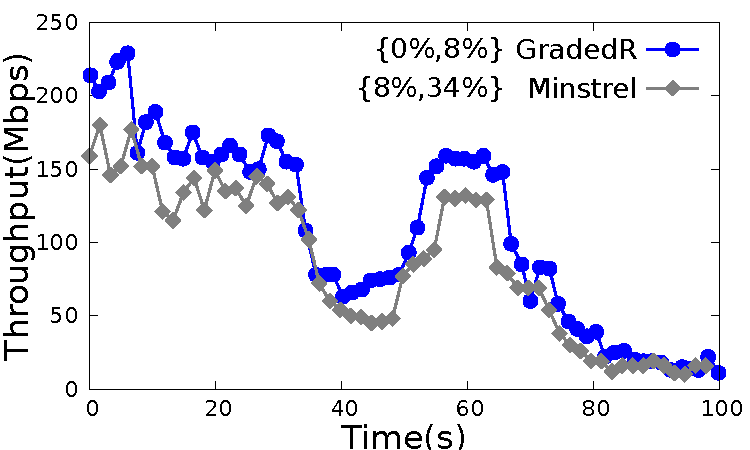
\includegraphics[width=3.6in]{chap3/route2.pdf}}
  \hspace{1in}
\centering
  \subfigure[3x3]{
  \label{fig:route3}
  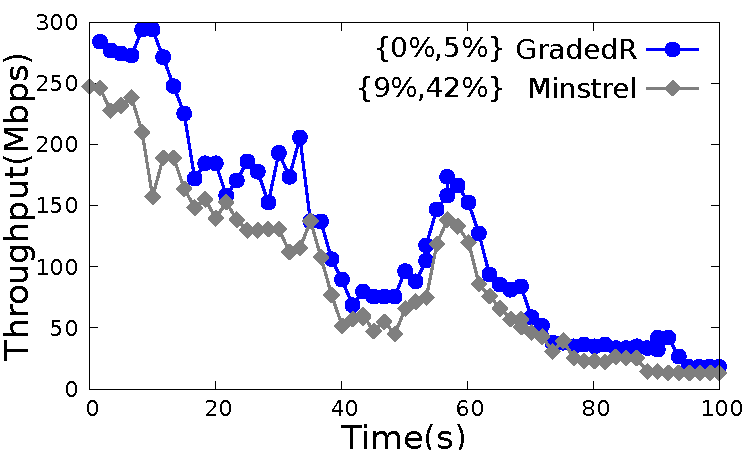
\includegraphics[width=3.6in]{chap3/route3.pdf}}
\bicaption[fig:route]{吞吐量及传输成功率}{吞吐量及传输成功率}{Fig}{Throughput improvements and PDR results along the route \textbf{r5}}
\end{figure}

\begin{figure}[!htp]
\centering
  \subfigure[1x3]{
  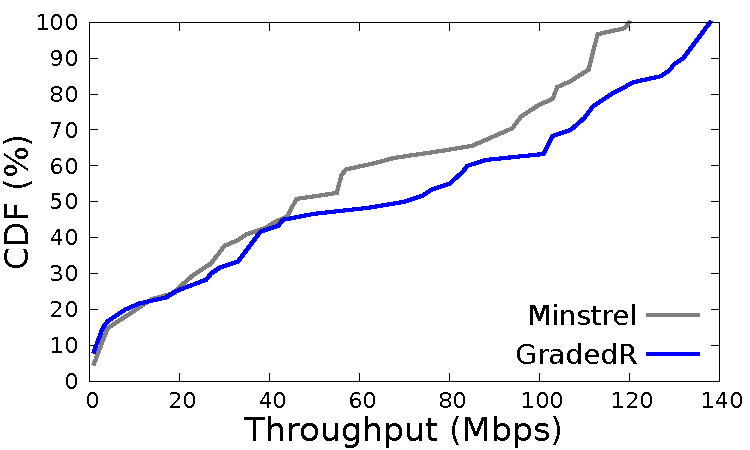
\includegraphics[width=3.6in]{chap3/CDF1x3.pdf}}
  \hspace{1in}
\centering
  \subfigure[2x3]{
  \includegraphics[width=3.6in]{chap3/CDF2x3.pdf}}
  \hspace{1in}
\centering
  \subfigure[3x3]{
  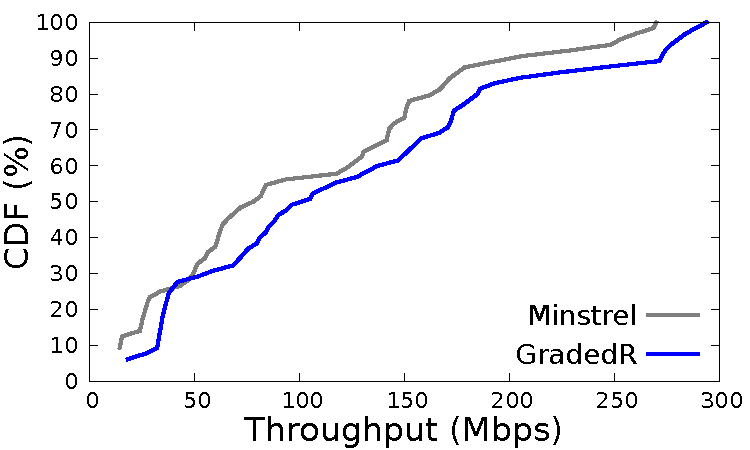
\includegraphics[width=3.6in]{chap3/CDF3x3.pdf}}
\bicaption[fig:cdfthr]{吞吐量累积分布函数}{吞吐量累积分布函数}{Fig}{CDF of throughput along the route \textbf{r5}}
\end{figure}

\begin{figure}[!htp]
\centering
  \subfigure[1x3]{
  \label{fig:thruput1}
  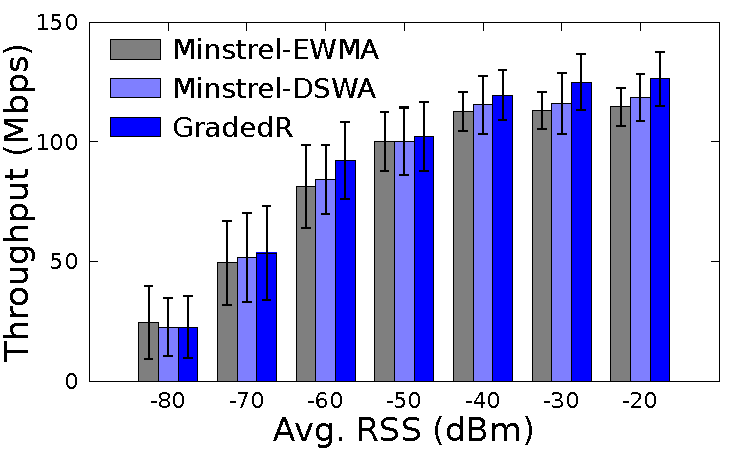
\includegraphics[width=3.6in]{chap3/goodput1.pdf}}
  \hspace{1in}
\centering
  \subfigure[2x3]{
  \label{fig:thruput2}
  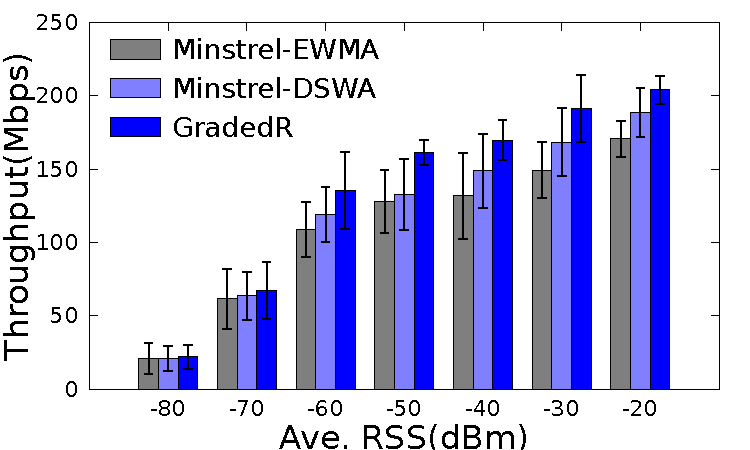
\includegraphics[width=3.6in]{chap3/goodput2.pdf}}
  \hspace{1in}
\centering
  \subfigure[3x3]{
  \label{fig:thruput3}
  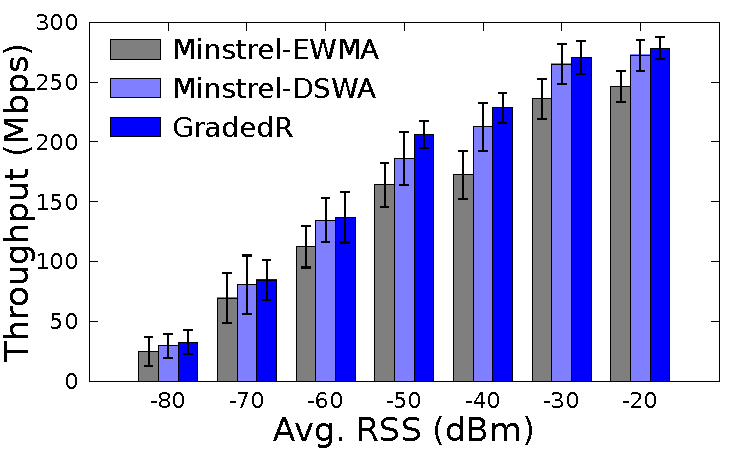
\includegraphics[width=3.6in]{chap3/goodput3.pdf}}
\bicaption[fig:throughput]{吞吐量及平均接收信号强度关系}{吞吐量及平均接收信号强度关系}{Fig}{Throughput vs. average RSS under different MIMO configurations}
\end{figure}

图 \ref{fig:route} 所示为沿线路\textbf{r5}(如图 \ref{fig:testbed80211n} 所示)的速率控制结果,主要对特定移动路线的PDR和吞吐量进行评估。首先对于所有的MIMO配置,GradedR能够明显提升网络可靠性,对于路线\textbf{r5}的所有GradedR测试至少91\%的PDR高于90\%,而Minstrel约有63\%的PDR低于90\%;同时随着MIMO可用天线数量的增加,GradedR的可靠性随之上升,其低于90\%的PDR所占比例由9\%降低为5\%,而Minstrel的这一比例却从37\% 上升为51\%,说明Minstrel的可靠性随着天线数量增加而降低。其次GradedR能够明显提高网络吞吐量,对于1$\times$3的MIMO配置,GradedR算法只有在时间20秒之前吞吐量高于Minstrel算法5-15Mbps,其他情况下的吞吐量基本相同;而在2$\times$3和3$\times$3的MIMO配置下,GradedR算法的吞吐量明显高于Minstrel算法,在2$\times$3配置下大约高于5-20Mbps,在3$\times$3配置下甚至达到30Mbps的性能提升。GradedR能够实现吞吐量的有效提升,一方面是由于上文中提到的PDR的大幅提升,另一方面在于其实时准确的配置选择策略。第一,GradedR利用DSWA算法能够获得准确的PDR参数,根据网络当前状态及在线PDR-RSS模型得到准确的最优配置选择,能够在保证网络可靠性的基础之上尽量提高网络吞吐量,而Minstrel 通过随机探测的方式寻找可用配置,或直接降低MCS\footnote{降低MCS值即降低网络的数据传输速率}以保证数据的可靠传输,其配置选择效率受到很大限制;第二,由于DSWA在网络状态稳定时能够有效降低测试开销,同时GradedR不需要多余的探测数据包进行测试,从而有效降低由配置选择带来的额外开销,而Minstrel需要依靠10\%的探测数据包来获得当前可用配置,其效率与准确性受到明显限制,同时探测数据包降低了可用数据传输的吞吐量。

吞吐量与平均RSS的关系如图 \ref{fig:throughput} 所示,包括图 \ref{fig:testbed80211n} 中\textbf{r1}到\textbf{r6}的所有移动测试数据。整体上GradedR能够在不同MIMO配置下实现更高的吞吐量,在相同的平均RSS条件下同样具有更高的吞吐量,同时吞吐量的提升随着天线数量和平均RSS的增加而增加。从图 \ref{fig:throughput} 可以看出,GradedR在1$\times$3和3$\times$3的MIMO配置下分别提升吞吐量5-15Mbps和10-40Mbps;在特定MIMO配置下,不同速率控制算法的吞吐量都与平均RSS密切相关,当平均RSS低于-60dBm时,单天线和双天线系统的吞吐量基本相同,GradedR在3$\times$3的MIMO系统下的最大吞吐量提升为5Mbps,主要原因是GradedR的可选配置受天线数量和平均RSS的限制。另一方面Minstrel速率控制算法结合DSWA测试算法同样可以实现吞吐量提升,相对于采用EWMA测试算法的Minstrel,Minstrel-DSWA的吞吐量提升同样随着天线数量和平均RSS而增加。如图 \ref{fig:throughput} 所示,当平均RSS高于-40dBm时,对于1$\times$3MIMO系统,Minstrel-DSWA能够获得最高8Mbps的吞吐量提升,对于2$\times$3 和3$\times$3MIMO系统,最高的吞吐量提升分别为25Mbps和30Mbps。总体上,在不同的MIMO配置条件下,GradedR相对于Minstrel能够实现40\%的吞吐量提升,同时在2$\times$3和3$\times$3的MIMO配置系统中,Minstrel算法结合DSWA测试算法同样能够实现高于Minstrel-EWMA算法20\%/25\%的吞吐量。


\section{本章小结}
\label{sec:conclusion3}

本章主要讨论在移动网络中,MIMO-OFDM无线系统的链路质量测试与建模问题。本文首先提出基于动态滑动窗口平均的PDR测试算法,通过数据包收发事件驱动确定采样间隔,从而避免多配置对PDR测试的影响,同时利用当前PDR信息降低测试开销。然后以PDR测试算法为基础,提出在线PDR-RSS建模框架,通过PDR-RSS模型数据库结合实时更新,解决MIMO-OFDM系统多配置带来的过渡窗口问题。以上的PDR测试算法与在线建模框架,通过同时应用物理层指标RSS与链路层指标PDR,有效地解决了移动性及多配置对链路质量测试与建模的影响。最后通过速率控制算法设计及其系统实现,对以上算法进行实验评估,评估结果表明本文提出的PDR测试算法能够提升89\%的测试精度,同时结合在线建模框架能够在不同MIMO配置下实现40\%的吞吐量提升。


\nocite{10.1109/TMC.2009.87,Ahmed2008Online,Deek:2011,dujovne2010taxonomy,hiertz2010802.11,kim2006accurate,kim2009experimental,kolar2011mesh}
\nocite{Pelechrinis2010high,perahia2008next,sevani2012sir,zhang2008practical,Zhao2003delivery}

\nocite{Balan:2012:AHD:2348543.2348552,Bhartia:2011:HFD:2030613.2030642,Chai:2012:BES:2348543.2348564,Gollakota:2011:CRS:2018436.2018456}
\nocite{Gudipati:2011:SAR:2018436.2018455,Magistretti:2011:WRW:2030613.2030619,Magistretti:2010:IML:1859995.1860030,Manweiler:2011:ARH:1999995.2000020}
\nocite{Nguyen:2011:OCD:2030613.2030624,Qian:2011:PRU:1999995.2000026,Rozner:2010:NNP:1814433.1814445,Sanadhya:2012:ACI:2348543.2348565}
